\documentclass[aspectratio=169]{beamer}
\usepackage{ctex, hyperref}
\usepackage{calligra}
\usepackage{pifont}
\usepackage{tikz}
\usepackage[T1]{fontenc}
\usepackage{SICNU}
% \usepackage[table]{xcolor}
\usepackage{bm}
\usepackage{subfigure}
\usepackage{ragged2e}
\usepackage{booktabs,makecell, multirow, tabularx}
\usepackage{float}
% \author{图灵的猫}
% \title{THU Beamer Theme}
% \subtitle{毕业设计开题报告}
% \institute{四川师范大学偏微分方程与物理团队}
\title[空间分数阶非线性薛定谔波动方程保结构算法研究
]{\small 空间分数阶非线性薛定谔波动方程保结构算法研究\\[2mm] 毕业设计}
\author[刘洋]{\footnotesize 汇报人:刘洋 \quad 导师:冉茂华 副教授}
\institute[四川师范大学偏微分方程与物理团队]{\footnotesize 四川师范大学偏微分方程与物理团队}
\date{\footnotesize \vskip -10pt \today}
% \date{2023年5月25日}
\usefonttheme[onlymath]{serif}%修改公式字体
\begin{document}

\kaishu
\begin{frame}
	\titlepage
	\vspace{-2mm}
	\begin{figure}[htpb]
		\begin{center}
			
\includegraphics[width=0.45\linewidth]{pic/SICNU_Logo2.png}
		\end{center}
	\end{figure}
\end{frame}
\begin{frame}
\tableofcontents[sectionstyle=show,subsectionstyle=show/shaded/hide,subsubsectionstyle=show/shaded/hide]
\end{frame}

\section{课题背景}
\begin{frame}{选题来源和论文类型}
	\begin{block}{非线性分数阶薛定谔波动方程(NFSWEs)}
		本课题主要考虑具有周期边界条件的 NFSWEs:
		\begin{equation}
			\left\{\begin{array}{l}
				u_{t t}+(-\Delta)^{\alpha / 2} u+\mathrm{i} \kappa u_t+\beta|u|^2 u=0,(\boldsymbol{x}, t) \in \mathbb{R}^d \times(0, T] \\
				u(\boldsymbol{x}, 0)=u_0(\boldsymbol{x}), u_t(\boldsymbol{x}, 0)=u_1(\boldsymbol{x}), \boldsymbol{x} \in \mathbb{R}^d
				\end{array}\right.\tag{8}
		\end{equation}
	  \end{block}

	  \begin{columns}
		\begin{column}{0.45\textwidth}
		  \begin{block}{选题来源}
			本研究为自选项目,选题源于分数阶微积分和非线性方程数值解法.
		  \end{block}
		\end{column}
		\begin{column}{0.45\textwidth}
		  \begin{block}{论文类型}
			本研究属于数值计算方向,是理论与实践相结合的应用型研究.	
		  \end{block}
		\end{column}
	  \end{columns}

\end{frame}

\begin{frame}{NFSWEs和守恒定律}
	\begin{block}{非线性分数阶薛定谔波动方程(NFSWEs)}
		本课题主要考虑具有周期边界条件的 NFSWEs:
		\begin{equation}
			\left\{\begin{array}{l}
				u_{t t}+(-\Delta)^{\alpha / 2} u+\mathrm{i} \kappa u_t+\beta|u|^2 u=0,(\boldsymbol{x}, t) \in \mathbb{R}^d \times(0, T] \\
				u(\boldsymbol{x}, 0)=u_0(\boldsymbol{x}), u_t(\boldsymbol{x}, 0)=u_1(\boldsymbol{x}), \boldsymbol{x} \in \mathbb{R}^d
				\end{array}\right.\tag{8}
		\end{equation}
		\vspace{-5mm}
		\begin{itemize}
		\item 质量守恒律
		\begin{equation}
			G(t)=\kappa\|u(\cdot, t)\|^2+2 \operatorname{Im}\left(u_t, u\right)\tag{9}
		\end{equation}
		\item 能量守恒律
		\begin{equation}\label{eq:10}
			E(t)=\left\|u_t(\cdot, t)\right\|^2+\left\|(-\Delta)^{\frac{\alpha}{4}} u(\cdot, t)\right\|^2+\frac{\beta}{2}\|u(\cdot, t)\|_{L^4}^4\tag{10}
		\end{equation}
	\end{itemize}
	  \end{block}
\end{frame}

\begin{frame}{研究意义}
	\begin{block}{非线性分数阶薛定谔波动方程(NFSWEs)}
		本课题主要考虑具有周期边界条件的 NFSWEs:
		\begin{equation}
			\left\{\begin{array}{l}
				u_{t t}+(-\Delta)^{\alpha / 2} u+\mathrm{i} \kappa u_t+\beta|u|^2 u=0,(\boldsymbol{x}, t) \in \mathbb{R}^d \times(0, T] \\
				u(\boldsymbol{x}, 0)=u_0(\boldsymbol{x}), u_t(\boldsymbol{x}, 0)=u_1(\boldsymbol{x}), \boldsymbol{x} \in \mathbb{R}^d
				\end{array}\right.\tag{8}
		\end{equation}
	  \end{block}

\begin{columns}
\begin{column}{0.45\textwidth}
	\begin{block}{研究价值}
	\begin{itemize}
		\setlength{\itemsep}{6pt}
		\item NFSWEs 应用背景
		\item 哈密顿结构
		\item 保结构算法
		\end{itemize}
	\end{block}
\end{column}
\begin{column}{0.45\textwidth}
	\begin{block}{研究难点}
	\begin{itemize}
		\setlength{\itemsep}{6pt}
		\item 非线性方程
		\item 波算子 $u_{tt} $
		\item 分数阶算子 $(-\Delta)^{\alpha / 2} u $
		\end{itemize}
	\end{block}
\end{column}
\end{columns}

\end{frame}

\section{研究现状}


\begin{frame}{国内外现状分析}
	% Table generated by Excel2LaTeX from sheet 'Sheet1'
	\begin{table}[htbp]
		\centering
		\small
		\caption{NFSWEs 国内外现状分析}
		  \begin{tabular}{lccccc}
		  \toprule
		  \textcolor[rgb]{0.227,0.373,0.306}{\textbf{文献}} & \textcolor[rgb]{0.227,0.373,0.306}{\textbf{维度}} & \textcolor[rgb]{0.227,0.373,0.306}{\textbf{空间精度}} & \textcolor[rgb]{0.227,0.373,0.306}{\textbf{时间精度}} & \textcolor[rgb]{0.227,0.373,0.306}{\textbf{能量守恒}} & \textcolor[rgb]{0.227,0.373,0.306}{\textbf{质量守恒}} \\
		  \midrule
		  \textcolor[rgb]{0.227,0.373,0.306}{\textbf{\cite{ranLinearlyImplicitConservative2016}{2016,Ran}}} & 1 维   & 2 阶   & 2 阶   & 修正能量  & 修正质量 \\
		  \midrule
		  \textcolor[rgb]{0.227,0.373,0.306}{\textbf{\cite{liFastEnergyConserving2018}{2018,Li}}} & 1 维   & 2 阶   & 2 阶   & 修正能量  & 修正质量 \\
		  \midrule
		  \textcolor[rgb]{0.227,0.373,0.306}{\textbf{\cite{panFourthorderDifferenceScheme2022}{2022,Pan}}} & 1 维   & 4 阶   & 2 阶   & 无     & 无 \\
		  \midrule
		  \textcolor[rgb]{0.227,0.373,0.306}{\textbf{\cite{chengConvergenceEnergyconservingScheme2022}{2022,Cheng}}} & 2 维   & 2 阶   & 2 阶   & 修正能量  & 无 \\
		  \midrule
		  \textcolor[rgb]{0.227,0.373,0.306}{\textbf{\cite{huEfficientEnergyPreserving2022}{2022,Hu}}} & 1 维   & 谱精度   & 2 阶   & 修正能量  & 无 \\
		  \midrule
		  \textcolor[rgb]{0.227,0.373,0.306}{\textbf{\cite{zhangHighorderStructurepreservingDifference2023}{2023,Zhang}}} & 1 维   & 4 阶   & 2 阶   & 修正能量  & 无 \\
		  \bottomrule
		  \end{tabular}%
		\label{tab:1}%
	  \end{table}%
		\end{frame}
	
		\begin{frame}{国内外现状分析}
			% Table generated by Excel2LaTeX from sheet 'Sheet1'
			\begin{table}[htbp]
				\centering
				\small
				\caption{NFSWEs 国内外现状分析}
				  \begin{tabular}{lccccc}
				  \toprule
				  \textcolor[rgb]{0.227,0.373,0.306}{\textbf{文献}} & \textcolor[rgb]{0.227,0.373,0.306}{\textbf{维度}} & \textcolor[rgb]{0.227,0.373,0.306}{\textbf{空间精度}} & \textcolor[rgb]{0.227,0.373,0.306}{\textbf{时间精度}} & \textcolor[rgb]{0.227,0.373,0.306}{\textbf{能量守恒}} & \textcolor[rgb]{0.227,0.373,0.306}{\textbf{质量守恒}} \\
				  \midrule
				  \textcolor[rgb]{0.227,0.373,0.306}{\textbf{\cite{ranLinearlyImplicitConservative2016}{2016,Ran}}} & 1 维   & 2 阶   & \textcolor{purple}{2 阶}   & \textcolor{purple}{修正能量}  & \textcolor{purple}{修正质量} \\
				  \midrule
				  \textcolor[rgb]{0.227,0.373,0.306}{\textbf{\cite{liFastEnergyConserving2018}{2018,Li}}} & 1 维   & 2 阶   & \textcolor{purple}{2 阶}   & \textcolor{purple}{修正能量}  & \textcolor{purple}{修正质量} \\
				  \midrule
				  \textcolor[rgb]{0.227,0.373,0.306}{\textbf{\cite{panFourthorderDifferenceScheme2022}{2022,Pan}}} & 1 维   & \textcolor{purple}{4 阶}   & \textcolor{purple}{2 阶}   & 无     & 无 \\
				  \midrule
				  \textcolor[rgb]{0.227,0.373,0.306}{\textbf{\cite{chengConvergenceEnergyconservingScheme2022}{2022,Cheng}}} & \textcolor{purple}{2 维}   & 2 阶   & \textcolor{purple}{2 阶}   & 修正能量  & 无 \\
				  \midrule
				  \textcolor[rgb]{0.227,0.373,0.306}{\textbf{\cite{huEfficientEnergyPreserving2022}{2022,Hu}}} & 1 维   & \textcolor{purple}{谱精度}   & \textcolor{purple}{2 阶}   & 修正能量  & 无 \\
				  \midrule
				  \textcolor[rgb]{0.227,0.373,0.306}{\textbf{\cite{zhangHighorderStructurepreservingDifference2023}{2023,Zhang}}} & 1 维   & 4 阶   & \textcolor{purple}{2 阶}   & 修正能量  & 无 \\
				  \bottomrule
				  \end{tabular}%
				\label{tab:2}%
			  \end{table}%
				\end{frame}
	
\begin{frame}{国内外现状分析}
\begin{exampleblock}{\footnotesize \cite{ranLinearlyImplicitConservative2016} \ M. Ran, C. Zhang, A linearly implicit conservative scheme for the fractional nonlinear Schrödinger equation with wave operator, Int J Comput Math. 93 {\color{purple}{(2016)}} 1103–1118.}
\footnotesize
% \vspace{-5mm}
\begin{itemize}
\item 空间方向:
\begin{equation*}
	\Delta_h^\gamma u_j^n=\frac{1}{h^\gamma} \sum_{k=1}^{M-1} g_{j-k}^{(\gamma)} u_k^n, \quad 1 \leq j \leq M-1
\end{equation*}
\item 时间方向:
\begin{equation*}
	\begin{gathered}
		\hat{v}_j^n=\frac{v_j^{n+1}+v_j^{n-1}}{2}, \quad \delta_t v_j^n=\frac{v_j^{n+1}-v_j^n}{\tau} \\
		\delta_{\hat{t}} v_j^n=\frac{v_j^{n+1}-v_j^{n-1}}{2 \tau}, \quad \delta_t^2 v_j^n=\frac{v_j^{n+1}-2 v_j^n+v_j^{n-1}}{\tau^2}
		\end{gathered}
\end{equation*}
\end{itemize}
\begin{columns}
\column{0.15\textwidth}
\begin{block}{\footnotesize 1 维}
\end{block}
\column{0.15\textwidth}
\begin{block}{\footnotesize 空间 2 阶}
\end{block}
\column{0.15\textwidth}
\begin{block}{\footnotesize 时间 2 阶}
\end{block}
\column{0.15\textwidth}
\begin{block}{\footnotesize 能量守恒\ \ding{51}}
\end{block}
\column{0.15\textwidth}
\begin{block}{\footnotesize 质量守恒\ \ding{51}}
\end{block}
\end{columns}

\end{exampleblock}
\end{frame}


	\begin{frame}{国内外现状分析}
		\begin{exampleblock}{\footnotesize \cite{liFastEnergyConserving2018} \ M. Li, Y.-L. Zhao, A fast energy conserving finite element method for the nonlinear fractional Schrödinger equation with wave operator, Appl Math Comput. 338 {\color{purple}{(2018)}} 758–773.}
			\footnotesize
			% \vspace{-5mm}
			\begin{itemize}
			\item 空间方向:
			\begin{equation*}
				\left(\delta_t^2 U^n, v_h\right)+B\left(\tilde{U}^n, v_h\right)+i \kappa\left(\delta_{\hat{t}} U^n, v_h\right)+\frac{\beta}{2}\left(\left(\left|U^{n+1}\right|^2+\left|U^{n-1}\right|^2\right) \tilde{U}^n, v_h\right)=0
			\end{equation*}
			\item 时间方向:
			\begin{equation*}
				\begin{aligned}
					\delta_t^2 v^n & =\frac{v^{n+1}-2 v^n+v^{n-1}}{\tau^2}, \quad \delta_t v^n=\frac{v^{n+1}-v^n}{\tau} \\
					\tilde{v}^n & =\frac{v^{n+1}+v^{n-1}}{2}, \quad \delta_{\hat{t}} v^n=\frac{v^{n+1}-v^{n-1}}{2 \tau}
					\end{aligned}
			\end{equation*}
		\end{itemize}
		\begin{columns}
			\column{0.15\textwidth}
			\begin{block}{\footnotesize 1 维}
			\end{block}
			\column{0.15\textwidth}
			\begin{block}{\footnotesize 空间 2 阶}
			\end{block}
			\column{0.15\textwidth}
			\begin{block}{\footnotesize 时间 2 阶}
			\end{block}
			\column{0.15\textwidth}
			\begin{block}{\footnotesize 能量守恒\ \ding{51}}
			\end{block}
			\column{0.15\textwidth}
			\begin{block}{\footnotesize 质量守恒\ \ding{51}}
			\end{block}
			\end{columns}
	
		\end{exampleblock}
		\end{frame}
				
	
\begin{frame}{国内外现状分析}
	\begin{exampleblock}{\footnotesize \cite{panFourthorderDifferenceScheme2022} \ K. Pan, J. Zeng, D. He, S. Zhang, A fourth-order difference scheme for the fractional nonlinear Schrödinger equation with wave operator, Appl Anal. 101 {\color{purple}{(2020)}} 2886–2902.}
		\footnotesize
		% \vspace{-5mm}
		\begin{itemize}
		\item 空间方向:
		\begin{equation*}
			\begin{gathered}
				\mathcal{A}_h^\alpha f(x)=\frac{\alpha}{24} f(x-h)+\left(1-\frac{\alpha}{12}\right) f(x)+\frac{\alpha}{24} f(x+h) \\
				\Delta_h^\alpha U_j=\mathcal{A}_h^\alpha\left((-\Delta)^{\frac{\alpha}{2}} U_j\right)+O\left(h^4\right) \\
				\mathcal{A}_h^\alpha \delta_t^2 U_j^n+i \mathcal{A}_h^\alpha \delta_{\hat{t}} U_j^n+\Delta_h^\alpha U_j^{\bar{n}}+\mathcal{A}_h^\alpha \beta\left|U_j^n\right|^2 U_j^{\bar{n}}+\mathcal{A}_h^\alpha \omega\left(x_j\right) U_j^{\bar{n}}=0
				\end{gathered}
		\end{equation*}
		\item 时间方向:
		\vspace{-2mm}
		\begin{equation*}
			\begin{gathered}
				P_j^{\bar{n}}=\frac{P_j^{n+1}+P_j^{n-1}}{2}, \quad \delta_t P_j^n=\frac{P_j^{n+1}-P_j^n}{\tau} \\
				\delta_{\hat{t}} P_j^n=\frac{P_j^{n+1}-P_j^{n-1}}{2 \tau}, \quad \delta_t^2 P_j^n=\frac{P_j^{n+1}-2 P_j^n+P_j^{n-1}}{\tau^2}
				\end{gathered}
		\end{equation*}
	\end{itemize}
	\vspace{-3mm}
	\begin{columns}
		\column{0.15\textwidth}
		\begin{block}{\footnotesize 1 维}
		\end{block}
		\column{0.15\textwidth}
		\begin{block}{\footnotesize 空间 4 阶}
		\end{block}
		\column{0.15\textwidth}
		\begin{block}{\footnotesize 时间 2 阶}
		\end{block}
		\column{0.15\textwidth}
		\begin{block}{\footnotesize 能量守恒\ \ding{55}}
		\end{block}
		\column{0.15\textwidth}
		\begin{block}{\footnotesize 质量守恒\ \ding{55}}
		\end{block}
		\end{columns}

	\end{exampleblock}
	\end{frame}


\begin{frame}{国内外现状分析}
	\begin{exampleblock}{\footnotesize \cite{chengConvergenceEnergyconservingScheme2022} \ X. Cheng, H. Qin, J. Zhang, Convergence of an energy-conserving scheme for nonlinear space fractional Schrödinger equations with wave operator, J Comput Appl Math. 400 {\color{purple}{(2022)}} 113762.}
		\footnotesize
		% \vspace{-5mm}
		\begin{itemize}
		\item 空间方向:
		\begin{equation*}
			\delta_x^\alpha v_j^n=-1 /(2 \cos (\alpha \pi / 2))\left(\delta_{x,+}^\alpha v_j^n+\delta_{x,-}^\alpha v_j^n\right)
		\end{equation*}
		\item 时间方向:
		\begin{equation*}
			\begin{aligned}
				& \delta_t U_j^{n+\frac{1}{2}}=V_j^{n+\frac{1}{2}}+R_1^n \\
				& \delta_t V_j^{n+\frac{1}{2}}=\partial_x^\alpha U_j^{n+\frac{1}{2}}-\mathrm{i} V_j^{n+\frac{1}{2}}-B^n W^{n+\frac{1}{2}}+Q_2^n \\
				& \delta_t W^{n+\frac{1}{2}}=\Re\left(B^n, \delta_t U^{n+\frac{1}{2}}\right)+R_3^n
				\end{aligned}
		\end{equation*}
	\end{itemize}
	\begin{columns}
		\column{0.15\textwidth}
		\begin{block}{\footnotesize 2 维}
		\end{block}
		\column{0.15\textwidth}
		\begin{block}{\footnotesize 空间 2 阶}
		\end{block}
		\column{0.15\textwidth}
		\begin{block}{\footnotesize 时间 2 阶}
		\end{block}
		\column{0.15\textwidth}
		\begin{block}{\footnotesize 能量守恒\ \ding{51}}
		\end{block}
		\column{0.15\textwidth}
		\begin{block}{\footnotesize 质量守恒\ \ding{55}}
		\end{block}
		\end{columns}
	
	\end{exampleblock}
	\end{frame}

\begin{frame}{国内外现状分析}
	\begin{exampleblock}{\footnotesize \cite{huEfficientEnergyPreserving2022} \ D. Hu, W. Cai, X.-M. Gu, Y. Wang, Efficient energy preserving Galerkin–Legendre spectral methods for fractional nonlinear Schrödinger equation with wave operator, Appl Numer Math. 172 {\color{purple}{(2022)}} 608–628.}
		\footnotesize
		% \vspace{-5mm}
		\begin{itemize}
		\item 空间方向:
		\begin{equation*}
			\begin{aligned}
				& \mathcal{A}(u, w)=\frac{1}{2 \cos \left(\frac{\pi x}{2}\right)}\left[\left({ }_a^{R L} D_x^{\alpha / 2} u,{ }_x^{R L} D_b^{\alpha / 2} w\right)+\left({ }_x^{R L} D_b^{\alpha / 2} u,{ }_a^{R L} D_x^{\alpha / 2} w\right)\right] \\
				& \left(u_t, w\right)=(v, w) \\
				& \left(v_t, w\right)+\mathcal{A}(u, w)+\mathrm{i} \kappa\left(u_t, w\right)+\beta\left(|u|^2 u, w\right)=0
				\end{aligned}
		\end{equation*}
		\item 时间方向:
		\begin{itemize}
			\item[1.] CN-GLS
			\vspace{-5mm}
		\begin{equation*}
			\begin{aligned}
				u^n & =u\left(x, t_n\right), \quad \delta_t u^{n+\frac{1}{2}}=\frac{u^{n+1}-u^n}{\tau} \\
				u^{n+\frac{1}{2}} & =\frac{u^{n+1}+u^n}{2}, \quad \tilde{u}^{n+\frac{1}{2}}=\frac{3 u^n-u^{n-1}}{2}
				\end{aligned}
		\end{equation*}
	\end{itemize}
\end{itemize}

	
	\end{exampleblock}
	\end{frame}
	
\begin{frame}{国内外现状分析}
	\begin{exampleblock}{\footnotesize \cite{huEfficientEnergyPreserving2022} \ D. Hu, W. Cai, X.-M. Gu, Y. Wang, Efficient energy preserving Galerkin–Legendre spectral methods for fractional nonlinear Schrödinger equation with wave operator, Appl Numer Math. 172 {\color{purple}{(2022)}} 608–628.}
		\footnotesize
		% \vspace{-5mm}
		\begin{itemize}
		\item 时间方向:
		\begin{itemize}
		\item[2.]SAV-GLS
		\vspace{-3mm}
		\begin{equation*}
			p(t)=\sqrt{\int_{\Omega} \frac{1}{2}|u|^4 d x+C_0} \quad \text { with } \quad \mathcal{F}(u)=\frac{|u|^2}{\sqrt{\int_{\Omega} \frac{1}{2}|u|^4 d x+C_0}}
		\end{equation*}
		\item[3.] ESAV-GLS
		\vspace{-3mm}
		\begin{equation*}
			q(t)=\exp \left(\int_{\Omega} \frac{1}{2}|u|^4 d x\right) \quad \text { with } \quad \mathcal{F}(u)=\frac{|u|^2}{\exp \left(\int_{\Omega} \frac{1}{2}|u|^4 d x\right)}
		\end{equation*}
	\end{itemize}
	\end{itemize}
	\vspace{-3mm}
	\begin{columns}
		\column{0.15\textwidth}
		\begin{block}{\footnotesize 1 维}
		\end{block}
		\column{0.15\textwidth}
		\begin{block}{\footnotesize 空间 谱精度}
		\end{block}
		\column{0.15\textwidth}
		\begin{block}{\footnotesize 时间 2 阶}
		\end{block}
		\column{0.15\textwidth}
		\begin{block}{\footnotesize 能量守恒\ \ding{51}}
		\end{block}
		\column{0.15\textwidth}
		\begin{block}{\footnotesize 质量守恒\ \ding{55}}
		\end{block}
		\end{columns}
	
	\end{exampleblock}
	\end{frame}


\begin{frame}{国内外现状分析}
	\begin{exampleblock}{\footnotesize \cite{zhangHighorderStructurepreservingDifference2023} \ X. Zhang, M. Ran, Y. Liu, L. Zhang, A high-order structure-preserving difference scheme for generalized fractional Schrödinger equation with wave operator, Math Comput Simulation. 210 {\color{purple}{(2023)}}  532–546.}
		\footnotesize
		% \vspace{-5mm}
		\begin{itemize}
		\item 空间方向:
		\begin{equation*}
			(-\Delta)^{\alpha / 2} u(x)=\frac{1}{h^\alpha} \sum_{k=-\infty}^{+\infty} \widehat{g}_k^{(\alpha)} u(x-k h)+O\left(h^4\right)
			\end{equation*}
			where
			\begin{equation*}
			\widehat{g}_k^{(\alpha)}=\left\{\begin{array}{l}
			\frac{4}{3} g_k^{(\alpha)}-\frac{1}{3 \cdot 2^\alpha} g_{\frac{k}{2}}^{(\alpha)}, k \text { is even } \\
			\frac{4}{3} g_k^{(\alpha)}, k \text { is odd }
			\end{array}\right.
			\end{equation*}
			in which
			\begin{equation*}
			g_k^{(\alpha)}=\left(1-\frac{\alpha+1}{\alpha / 2+k}\right) g_{k-1}^{(\alpha)} \text { and } g_0^{(\alpha)}=\frac{\Gamma(\alpha+1)}{\Gamma^2(\alpha / 2+1)}, k=1,2, \ldots
			\end{equation*}
			\end{itemize}
	\end{exampleblock}
	\end{frame}

	\begin{frame}{国内外现状分析}
		\begin{exampleblock}{\footnotesize \cite{zhangHighorderStructurepreservingDifference2023} \ X. Zhang, M. Ran, Y. Liu, L. Zhang, A high-order structure-preserving difference scheme for generalized fractional Schrödinger equation with wave operator, Math Comput Simulation. 210 {\color{purple}{(2023)}}  532–546.}
			\footnotesize
			% \vspace{-5mm}
			\begin{itemize}
			\item 时间方向:
				
			TSAV
		\begin{equation*}
		r(t)=\sin \left(E_1(u)\right)+\varepsilon, \quad \text { where } \quad E_1(u)=\int_{\Omega} F\left(|u|^2\right) d x
		\end{equation*}
		$\mathrm{CN}$ 格式\&外推公式
		\begin{equation*}
		\begin{aligned}
		\delta_t v_j^{n+\frac{1}{2}} & =\frac{v_j^{n+1}-v_j^n}{\tau}, \quad \delta_x v_j^n=\frac{v_{j+1}^n-v_j^n}{h}, \\
		v_j^{n+\frac{1}{2}} & =\frac{v_j^{n+1}+v_j^n}{2}, \quad \tilde{v}_j^{n+\frac{1}{2}}=\frac{3 v_j^n-v_j^{n-1}}{2} .
		\end{aligned}
		\end{equation*}
		\end{itemize}
		\begin{columns}
			\column{0.15\textwidth}
			\begin{block}{\footnotesize 1 维}
			\end{block}
			\column{0.15\textwidth}
			\begin{block}{\footnotesize 空间 4 阶}
			\end{block}
			\column{0.15\textwidth}
			\begin{block}{\footnotesize 时间 2 阶}
			\end{block}
			\column{0.15\textwidth}
			\begin{block}{\footnotesize 能量守恒\ \ding{51}}
			\end{block}
			\column{0.15\textwidth}
			\begin{block}{\footnotesize 质量守恒\ \ding{55}}
			\end{block}
			\end{columns}
		
		\end{exampleblock}
		\end{frame}

\section{研究内容}
\begin{frame}{课题研究目标}
	本课题的目标是为二维NFSWEs构建:
	\begin{itemize}
		\item 任意高阶显式保结构数值格式.
		\item 能够同时保持原始能量和原始质量守恒的数值格式.
	\end{itemize}
% \begin{table}[htbp]
% 	\centering
% 	% \caption{本课题的目标是为二维NFSWEs构建高效的显式保结构格式以及能够同时保持原始能量和质量的格式}
% 	  \begin{tabular}{cccccc}
% 	  \toprule
% 	  \textcolor[rgb]{0.227,0.373,0.306}{} & \textcolor[rgb]{0.227,0.373,0.306}{\textbf{维度}} & \textcolor[rgb]{0.227,0.373,0.306}{\textbf{空间精度}} & \textcolor[rgb]{0.227,0.373,0.306}{\textbf{时间精度}} & \textcolor[rgb]{0.227,0.373,0.306}{\textbf{能量守恒}} & \textcolor[rgb]{0.227,0.373,0.306}{\textbf{质量守恒}} \\
% 	  \midrule
% 	  \textcolor[rgb]{0.227,0.373,0.306}{\textbf{研究目标-1}} & \textcolor{purple}{2 维}   & \textcolor{purple}{谱精度}   & \textcolor{purple}{任意高阶}  & 修正能量  & 无 \\
% 	  \midrule
% 	  \textcolor[rgb]{0.227,0.373,0.306}{\textbf{研究目标-2}} & \textcolor{purple}{2 维}   & \textcolor{purple}{谱精度}   & 2 阶   & \textcolor{purple}{原始能量}  & \textcolor{purple}{原始质量} \\
% 	  \bottomrule
% 	  \end{tabular}%
% 	\label{tab:3}%
%   \end{table}%

\end{frame}

\begin{frame}{研究内容及其可行性研究}
	\begin{block}{任意高阶显式保结构数值格式}
		\textbf{\textcolor[rgb]{0.227,0.373,0.306}{研究内容:}}
		
		{\footnotesize 本课题拟通过将IEQ方法或SAV方法与显式RRK方法结合,为二维空间分数阶非线性薛定谔波动方程构造一类任意高阶显式守恒格式.}
		
		\textbf{\textcolor[rgb]{0.227,0.373,0.306}{可行性分析:}}
		\begin{itemize}
			\item {\footnotesize Ketcheson\cite{ketchesonRelaxationRungeKutta2019}提出了松弛龙格-库塔(RRK)方法,该方法可以为任何二次不变量构建显式的守恒格式.}%随后,RRK 技术被扩展到一般凸不变量 \cite{ranochaRelaxationRungeKutta2020}.}
			\item {\footnotesize 不变能量二次方化 (IEQ) 方法 \cite{yangLinearUnconditionallyEnergy2017, yangEfficientLinearSchemes2017}和标量辅助变量 (SAV) 方法 \cite{chengConvergenceEnergyconservingScheme2022} 可以通过变量变换将能量\eqref{eq:10}转换为新变量的二次形式.}
			\end{itemize}
	\end{block}
	\end{frame}



\begin{frame}{研究内容及其可行性研究}
	\begin{block}{同时保持原始能量和原始质量守恒的数值格式}
		\textbf{\textcolor[rgb]{0.227,0.373,0.306}{研究内容:}}
		
		{\footnotesize 本课题拟首先通过分数阶Laplacian泛函的变分导数将NFSWEs重新表述为哈密顿系统.然后结合PAVF系列方法为二维NFSWEs构造能够同时保原始能量和原始质量的守恒格式.}
		
		\textbf{\textcolor[rgb]{0.227,0.373,0.306}{可行性分析:}}
		\begin{itemize}
			\item {\footnotesize PAVF方法可以守恒除常规能量之外的更多守恒性质,并已被用于构造哈密顿常微分方程的守恒格式\cite{caiPartitionedAveragedVector2018}.​​​​​​​​​​​​​​​​​​​​​​​​​​​​​​​​​​​​​​​​​​​​​​​​​​​​​​​​​​​​​​​​​​​​​​​​​​​​​​​​​​​​​​​​​​​​​​​​​​​​​​​​​​​​​​​​​​​​​​​​​​​​​​​​​​​​​​​​​​​​​​​​​​​​​​​​​​​​​​​​​​​​​​​​​​​​​​​​​​​​​​​​​​​​​​​​​​​​​​​​​​​​​​​​​​​​​​​​​​​​​​​​​​​​​​​​​​​​​​​​​​​​​​​​​​​​​​​​​​​​​​​​​​​​​​​​​​​​​​​​​​​​​​​​​​​​​​​​​​​​​​​​​​​​​​​​​​​​​​​​​​}
			\item {\footnotesize Wang 和 Huang \cite{wangStructurepreservingNumericalMethods2018} 提出了分数阶Laplacian泛函的变分导数并将一维分数阶非线性Schrödinger方程重新表述为哈密顿系统.Fu 和 Cai \cite{fuStructurepreservingAlgorithmsTwodimensional2020} 推导了二维分数阶 Klein-Gordon-Schrödinger 方程的哈密顿公式,并随后构建了守恒格式.}
			\end{itemize}
	\end{block}
	\end{frame}
	
\begin{frame}{拟解决的关键问题与实施方案}
	\begin{block}{拟解决的关键问题}
		{\footnotesize 通过对关键问题的深入研究,可以为二维NFSWEs的数值求解和数值模拟提供有效的数值方法和理论支持,对相关领域的应用和理论研究具有重要的参考价值和实际意义.}
		\begin{itemize}
		\item {\footnotesize \textbf{\textcolor[rgb]{0.227,0.373,0.306}{空间半离散格式构造(傅立叶伪谱方法):}}充分利用傅立叶变换的优势并使用快速傅立叶变换(FFT)算法,获得高精度和高效率的数值近似.}
		\item {\footnotesize \textbf{\textcolor[rgb]{0.227,0.373,0.306}{松弛系数的显式计算格式推导:}}通过对松弛参数的准确计算,确保数值方法能够保持方程所需的物理特性.}
		\item {\footnotesize \textbf{\textcolor[rgb]{0.227,0.373,0.306}{哈密顿系统的建立:}}为了构建保持原始质量和能量守恒的数值方法,需要对问题的哈密顿结构进行推导.}
		\item {\footnotesize \textbf{\textcolor[rgb]{0.227,0.373,0.306}{守恒性质的证明及精度分析:}}守恒性质的证明及精度分析将帮助评估数值方法的准确性和可靠性,为二维NFSWEs的数值模拟提供重要的理论支持. 同时有助于对数值方法进行改进和优化,以提高其性能和适用性.}
		% \item {\footnotesize \textbf{\textcolor[rgb]{0.227,0.373,0.306}{数值方法的实现和数值实验验证:}}设计好数值方法后,需要进行一系列的数值实验来验证该方法的有效性和可靠性.同时需要与其他数值方法进行比较,以便更加客观地评估所提出的数值方法的性能和优势.}
		\end{itemize}
	\end{block}
	\end{frame}

\begin{frame}{拟解决的关键问题与实施方案}
	\begin{block}{实施方案}
		{\footnotesize 针对以上拟采取的研究方法,可以考虑以下具体可操作的实施方案:}
		\begin{itemize}
		\item {\footnotesize \textbf{\textcolor[rgb]{0.227,0.373,0.306}{文献研究:}}明确研究范围和领域,建立文献库,使用专业数据库和搜索引擎筛选与研究主题相关的最新成果.利用Zotero进行文献管理和分析,形成系统性的文献综述,确定理论基础和前沿动态.}
		\item {\footnotesize \textbf{\textcolor[rgb]{0.227,0.373,0.306}{数学理论分析:}}基于文献综述,深入研究分数阶微积分、Fourier变换、哈密顿系统等数学概念,建立相关模型.探究IEQ、SAV、RRK和PAVF方法的数学原理、计算效果,通过符号、公式、图表清晰表达分析思路和结论.}
		\item {\footnotesize \textbf{\textcolor[rgb]{0.227,0.373,0.306}{数值计算模拟:}}设计算法和计算模拟格式,选择适当参数,通过有效性和稳定性测试验证计算程序.对计算结果进行可视化和分析,参考领域研究成果,进行优化和改进格式探索.注意误差来源和控制方法,确保研究成果的准确性和可靠性.}
		\end{itemize}
	\end{block}
	\end{frame}


	\section{Numerical examples}
	\begin{frame}%\frametitle{Numerical examples}
	%In this section, we carry out several numerical experiments to illustrate the accuracy and conservation
	%property of the explicit SAV-RRK methods \eqref{eq:4-3}. Also some comparisons with other classical explicit SAV-RK methods are supported.
	%%It is important to mention that a fast solver method utilizing the fast Fourier transformation (FFT) technique is employed for calculations, effectively reducing memory requirements and computational complexity.
	\footnotesize Without loss of generality, the following explicit RK methods will be used in calculation.
	%\end{frame}
	%
	%\begin{frame}\small
	  \begin{enumerate}
		\item $\operatorname{RK}(2,2)$ : two-stage, second order Heun method %of \cite{shuEfficientImplementationEssentially1988}.
		\begin{equation}
		\begin{array}{c|cc}
		0 & 0 & 0 \\
		\frac{2}{3} & \frac{2}{3} & 0 \\
		\hline & \frac{1}{4} & \frac{3}{4}
		\end{array}
		\end{equation}
	
		\item $\mathrm{RK}(3,3)$ : three-stage, third order Heun method %of \cite{shuEfficientImplementationEssentially1988}.
	
		\begin{equation}
		\begin{array}{c|ccc}
		0 & 0 & 0 & 0 \\
		\frac{1}{3} & \frac{1}{3} & 0 & 0 \\
		\frac{2}{3} & 0 & \frac{2}{3} & 0 \\
		\hline & \frac{1}{4} & 0 & \frac{3}{4}
		\end{array}
		\end{equation}
	
		\item $\operatorname{RK}(4,4)$ : four-stage, fourth order Gill method %of \cite{shuEfficientImplementationEssentially1988}.
	
		\begin{equation}
		\begin{array}{c|cccc}
		0 & 0 & 0 & 0 & 0 \\
		\frac{1}{2} & \frac{1}{2} & 0 & 0 & 0 \\
		\frac{1}{2} & \frac{\sqrt{2}-1}{2} & 1-\frac{\sqrt{2}}{2} & 0 & 0 \\
		1 & 0 & -\frac{\sqrt{2}}{2} & 1+\frac{\sqrt{2}}{2} & 0 \\
		\hline & \frac{1}{6} & \frac{2-\sqrt{2}}{6} & \frac{2+\sqrt{2}}{6} & \frac{1}{6}
		\end{array}
		\end{equation}
		\end{enumerate}
	\end{frame}
	%\begin{frame}\small
	%It is worth noting that the main focus of this work is accuracy in
	%temporal. Therefore, the spectral accuracy phenomenon presented in spatial is not shown.
	%Additionally, given the inherent positivity of the energy in our numerical examples, we consistently set the constant $C_0$ as zero to ensure energy positivity
	%% It is worth noting that we have verified that the spatial orientation is spectrally accurate, we just did not explicitly demonstrate the spatial accuracy.
	%
	%The errors and the convergence order in Temporal are calculated by
	%\begin{equation}
	%	Error(\tau)=\left\|U_{N}^{M}-U_{N}^{2 M}\right\|_{\infty},~\text { order }=\log _{2}[Error(\tau) / Error(\tau / 2)].\label{eq_104}
	%\end{equation}
	%In order to depict the conservation performance, the relative error of energy is calculated by
	%\begin{equation}\label{eq_105}
	%R E_{\gamma}^{m}=\left|\left(E_{\gamma}^{m}-E_{\gamma}^{0}\right) / E_{\gamma}^{0}\right|,
	%\end{equation}
	%where $E_{\gamma}^{m}$ denotes the discrete energy at $t_m$.
	%\end{frame}
	
	\begin{frame}\frametitle{Numerical examples: 1D NFSWEs}
	  \begin{example}\label{ex:1}
	  \footnote{\tiny 	M.~Ran, C.~Zhang,
	  \href{http://www.tandfonline.com/doi/full/10.1080/00207160.2015.1016924}{A
	  linearly implicit conservative scheme for the fractional nonlinear
	  {{Schr\"odinger}} equation with wave operator}, Int. J. Comput. Math. 93~(7)
	  (2016) 1103--1118.
	} First, we consider 1D NFSWEs \eqref{eq_1}-\eqref{eq_3} as
	  \begin{equation}\label{eq_108}
	  u_{t t}+(-\Delta)^{\alpha / 2} u+\mathrm{i}u_t+|u|^2 u=0, \quad (x,t)\in  (-25, 25)\times[0, T],
	  \end{equation}
	  with $u(x, 0)=(1+\mathrm{i}) x e^{-10(1-x)^2}$ and $u_t(x, 0)=0$.
	  \end{example}
	
	Without loss of generality, here we set $\alpha=1.5$ and $T=1$ to confirm the accuracy of the explicit SAV-RRK methods \eqref{eq:4-3}.
	\end{frame}
	
	
	
	\begin{frame}\frametitle{Numerical examples: 1D NFSWEs}
	\begin{table}[H]\tiny
	  \centering
	  \caption{Numerical errors and convergence order in time for Example \ref{ex:1} when $N=32, T = 1$.}
	  \begin{tabular}{lllllrlrlrlrlrl}
	  \toprule
	  \multicolumn{2}{l}{\multirow{2}[3]{*}{\textbf{RK(Stage,Order)}}} & \multicolumn{2}{l}{\multirow{2}[3]{*}{$\bm{\tau}$}} & \multicolumn{3}{c}{\textbf{SAV-RK}} &       & \multicolumn{3}{c}{\textbf{SAV-RRK(RT)}} &       & \multicolumn{3}{c}{\textbf{SAV-RRK(IDT)}} \\
	  \cmidrule{5-7}\cmidrule{9-11}\cmidrule{13-15}    \multicolumn{2}{l}{} & \multicolumn{2}{l}{} & \textbf{Error($\tau$)} &       & \textbf{order} &       & \textbf{Error($\tau$)} &       & \textbf{order} &       & \textbf{Error($\tau$)} &       & \textbf{order} \\
	  \hline
	  \multicolumn{2}{l}{\multirow{5}[0]{*}{\textbf{RK(2,2)}}} & \multicolumn{2}{l}{0.1} & 1.8552E-04 &       & -     &       & 1.9063E-04 &       & -     &       & 2.0325E-04 &       & - \\
	  \multicolumn{2}{l}{} & \multicolumn{2}{l}{0.05} & 4.6601E-05 &       & 1.9931  &       & 4.7240E-05 &       & 2.0126  &       & 5.0585E-05 &       & 2.0065  \\
	  \multicolumn{2}{l}{} & \multicolumn{2}{l}{0.025} & 1.1671E-05 &       & 1.9974  &       & 1.1750E-05 &       & 2.0074  &       & 1.2387E-05 &       & 2.0298  \\
	  \multicolumn{2}{l}{} & \multicolumn{2}{l}{0.0125} & 2.9200E-06 &       & 1.9990  &       & 2.9294E-06 &       & 2.0040  &       & 2.9549E-06 &       & 2.0677  \\
	  \multicolumn{2}{l}{} & \multicolumn{2}{l}{0.00625} & 7.3022E-07 &       & 1.9996  &       & 7.3130E-07 &       & 2.0021  &       & 6.6665E-07 &       & 2.1481  \\
	  \multicolumn{2}{l}{\multirow{5}[0]{*}{\textbf{RK(3,3)}}} & \multicolumn{2}{l}{0.1} & 7.6862E-06 &       & -     &       & 2.9857E-06 &       & -     &       & 1.7245E-04 &       & - \\
	  \multicolumn{2}{l}{} & \multicolumn{2}{l}{0.05} & 9.5269E-07 &       & 3.0122  &       & 3.9037E-07 &       & 2.9352  &       & 4.3389E-05 &       & 1.9907  \\
	  \multicolumn{2}{l}{} & \multicolumn{2}{l}{0.025} & 1.1866E-07 &       & 3.0052  &       & 5.0077E-08 &       & 2.9626  &       & 1.0873E-05 &       & 1.9966  \\
	  \multicolumn{2}{l}{} & \multicolumn{2}{l}{0.0125} & 1.4809E-08 &       & 3.0023  &       & 6.3449E-09 &       & 2.9805  &       & 2.7208E-06 &       & 1.9986  \\
	  \multicolumn{2}{l}{} & \multicolumn{2}{l}{0.00625} & 1.8497E-09 &       & 3.0011  &       & 7.9858E-10 &       & 2.9901  &       & 6.8049E-07 &       & 1.9994  \\
	  \multicolumn{2}{l}{\multirow{5}[1]{*}{\textbf{RK(4,4)}}} & \multicolumn{2}{l}{0.1} & 3.7701E-07 &       & -     &       & 3.8894E-07 &       & -     &       & 7.0733E-07 &       & - \\
	  \multicolumn{2}{l}{} & \multicolumn{2}{l}{0.05} & 2.3572E-08 &       & 3.9994  &       & 2.3939E-08 &       & 4.0221  &       & 4.4585E-08 &       & 3.9878  \\
	  \multicolumn{2}{l}{} & \multicolumn{2}{l}{0.025} & 1.4730E-09 &       & 4.0003  &       & 1.4843E-09 &       & 4.0115  &       & 2.8080E-09 &       & 3.9889  \\
	  \multicolumn{2}{l}{} & \multicolumn{2}{l}{0.0125} & 9.2041E-11 &       & 4.0003  &       & 9.2397E-11 &       & 4.0058  &       & 1.7743E-10 &       & 3.9842  \\
	  \multicolumn{2}{l}{} & \multicolumn{2}{l}{0.00625} & 5.7518E-12 &       & 4.0002  &       & 5.7630E-12 &       & 4.0029  &       & 1.1309E-11 &       & 3.9718  \\
	  \bottomrule
	  \end{tabular}%
	  \label{tab:6-1}%
	  \end{table}%
	\end{frame}
	
	
	\begin{frame}\frametitle{Numerical examples: 1D NFSWEs}
	From Table \ref{tab:6-1}, we can see that
	\begin{itemize}
	  \item All SAV-RRK(RT) methods keep the same convergence order as the standard SAV-RK methods while the SAV-RRK(IDT) methods behave differently.
	  \item The SAV-RRK(IDT)(2,2) and SAV-RRK(IDT)(4,4) give convergence order  which are higher than the expected orders as indicated in Theorem \ref{thm:5_4} while SAV-RRK(IDT)(3,3) give convergence order reduced by one.
	  \item This different behavior could be attributed to the convergence order of $\max\limits _m\left|\gamma_m-1\right|$ get improved by one order for SAV-RRK(RT)(2, 2) and SAV-RRK(RT)(4, 4) as displayed in Fig. \ref{fig:1}.
	\end{itemize}
	\end{frame}
	
	\begin{frame}\footnotesize
	%Furthermore, we conduct an investigation into the relaxation coefficient $\gamma_m$ at each step.
	Also, we calculate $\max\limits _m\left|\gamma_m-1\right|$ and $\max\limits _m\left|S_m(1)\right|$ with different time step $\tau$.
	%The numerical results for some relaxation methods are displayed in Fig. \ref{fig:1}:
	\begin{figure}[H]
	  \begin{center}
	  \subfigure[$\max\limits_m\left|\gamma_m-1\right|$]{ \centering
	  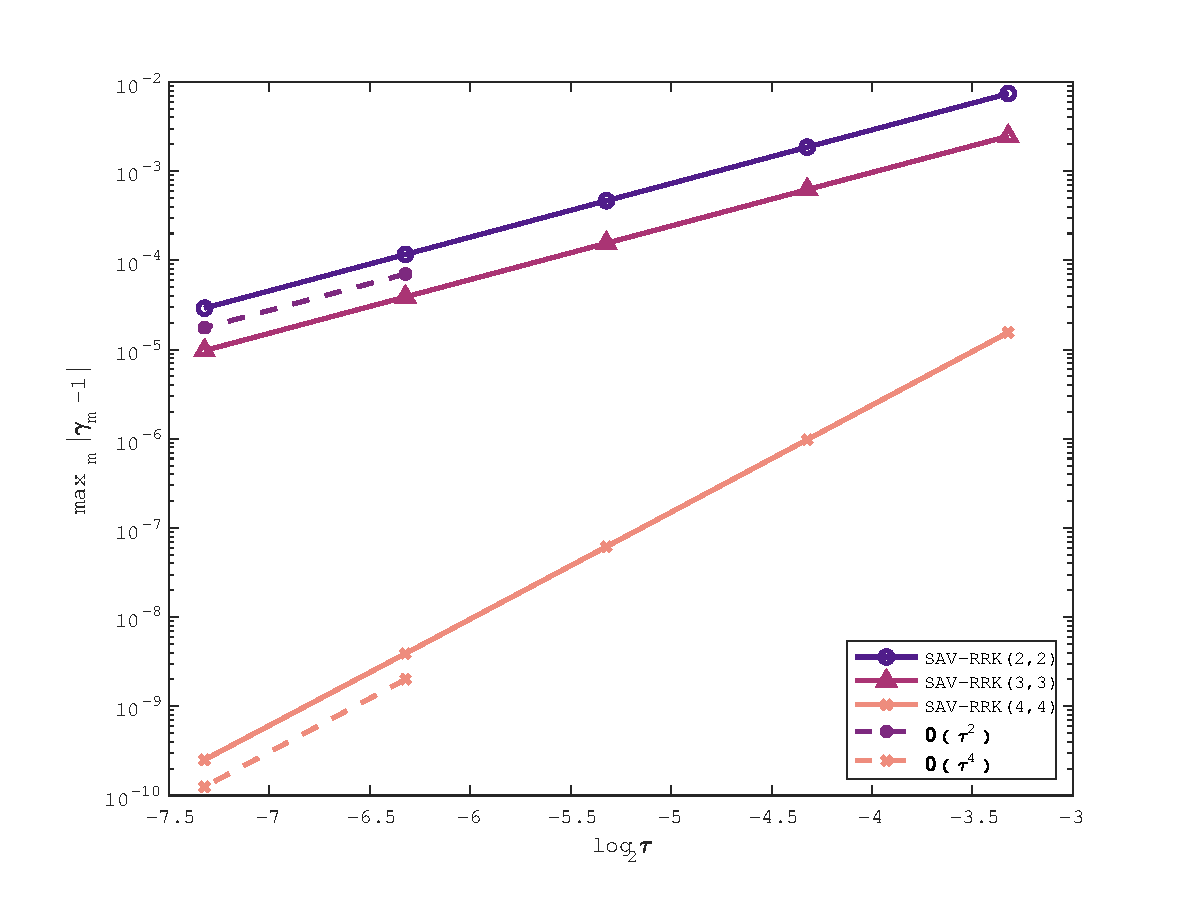
\includegraphics[width=0.45\textwidth]{./figure/exp1_r.eps}
	  %\centerline{($b$) Spatial accuracy with $\tau = 10^{-3}.$}
	  }\subfigure[$\max\limits_m\left|S_m(1)\right|$]{ \centering
	  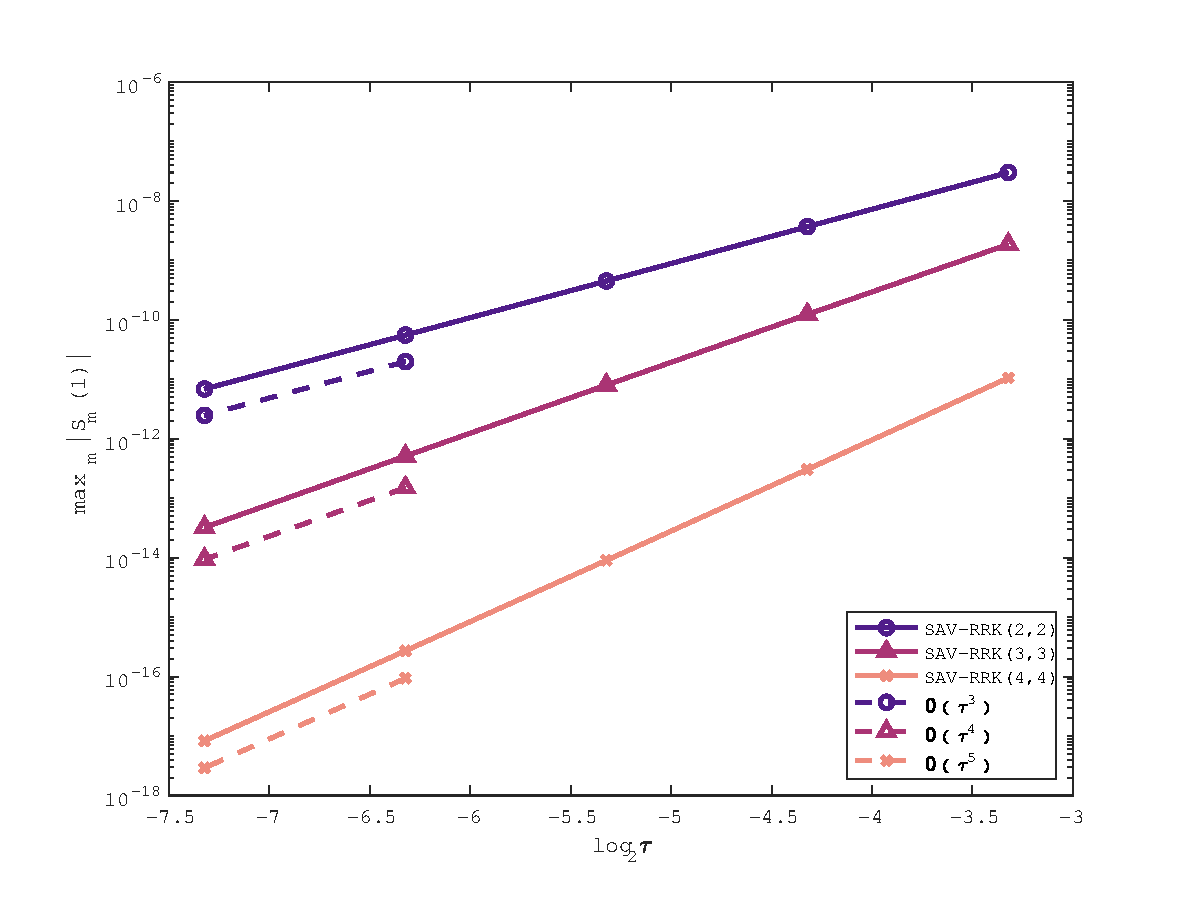
\includegraphics[width=0.45\textwidth]{./figure/exp1_s.eps}
	  %\centerline{($a$) Temporal accuracy with $N=128.$}
	  }\caption{$\max\limits_m\left|\gamma_m-1\right|$ and $\max\limits_m\left|S_m(1)\right|$ for some relaxation methods in Example \ref{ex:1}.}
	  \label{fig:1}
	  \end{center}
	  \end{figure}
	One can see that the orders of the above two quantities are consistent with the theoretical results in Lemma \ref{lem:5_1} and Theorem \ref{thm:5_1}.  It is worth noting that some similar results can be obtained when varying the value of $\alpha$, although these phenomena are not shown here.
	\end{frame}
	
	\begin{frame}\frametitle{Numerical examples: 1D NFSWEs}
	We also run a long time simulation till $T=1000$ and plot the relative energy by the SAV-RRK(4,4) methods with different $\alpha$ in Fig. \ref{fig:4},
	which indicates that the proposed schemes can preserve the energy exactly in discrete level and the conservation performance is significantly better
	than the SAV method \footnote{\tiny X.~Cheng, H.~Qin, J.~Zhang,
	\href{https://linkinghub.elsevier.com/retrieve/pii/S0377042721003848}{Convergence
	of an energy-conserving scheme for nonlinear space fractional
	{{Schr\"odinger}} equations with wave operator}, J. Comput. Appl. Math. 400
	(2022) 113762.
	} and three-level linearly implicit difference method\footnote{\tiny 	P.~Wang, C.~Huang, \href{https://doi.org/10.1007/s11075-014-9917-x}{A
	conservative linearized difference scheme for the nonlinear fractional
	{{Schr\"odinger}} equation}, Numer. Algorithms 69~(3) (2015) 625--641.}.
	\end{frame}
	
	\begin{frame}
	  \vspace{-3mm}
	  \begin{figure}[H]
		\begin{center}
		\subfigure[$\alpha=1.3$]{ \centering
		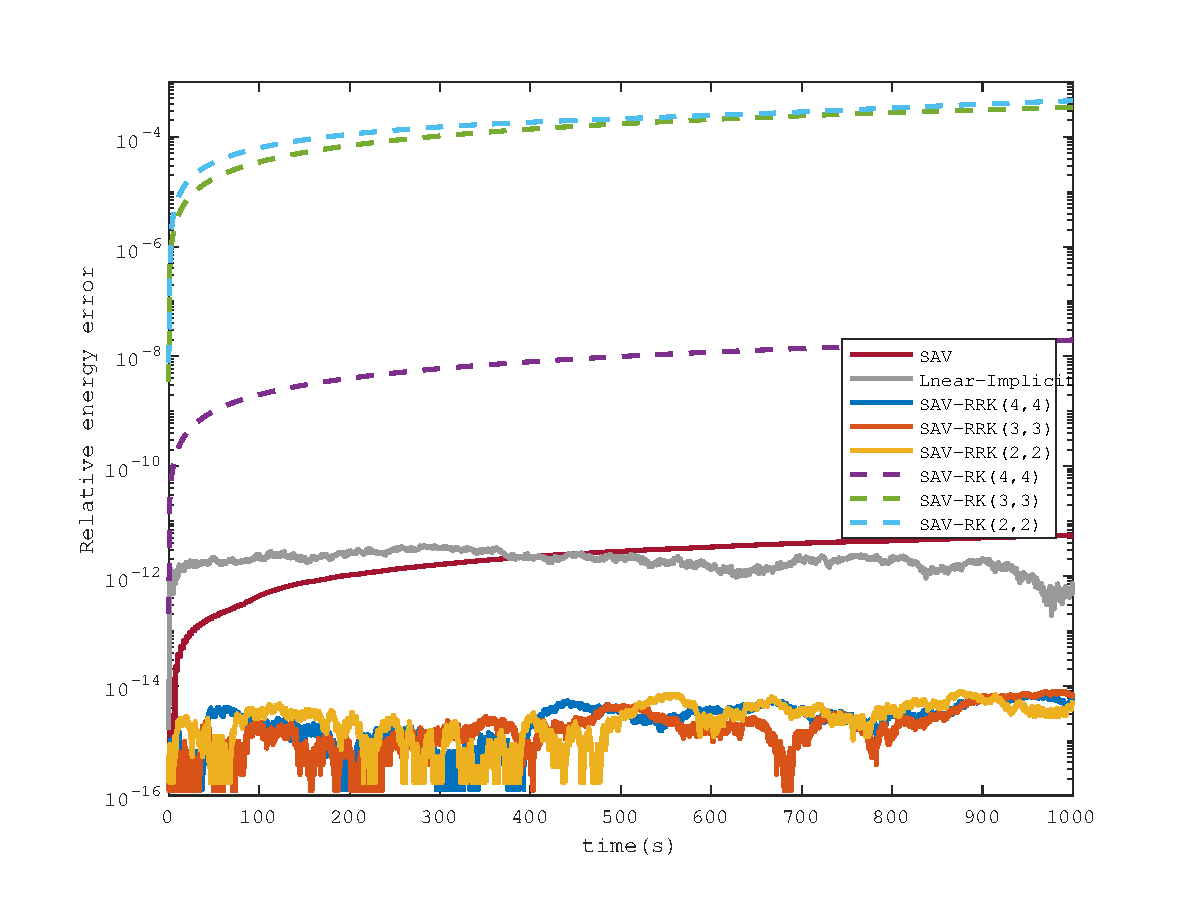
\includegraphics[width=0.35\textwidth]{./figure/exp1_energy3.eps}
		%\centerline{($b$) Spatial accuracy with $\tau = 10^{-3}.$}
		}\subfigure[$\alpha=1.6$]{ \centering
		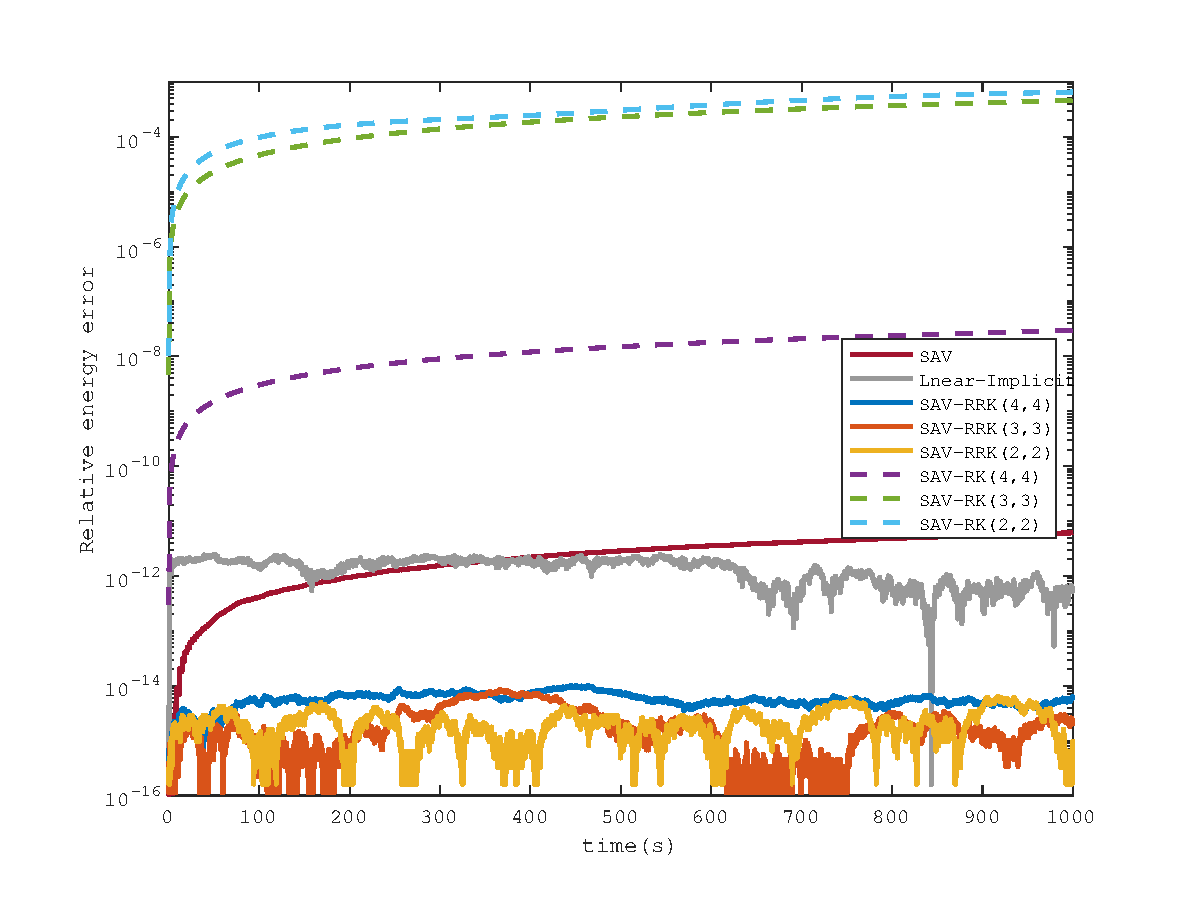
\includegraphics[width=0.35\textwidth]{./figure/exp1_energy6.eps}
		%\centerline{($a$) Temporal accuracy with $N=128.$}
		}\\ \vspace{-3mm}
		\subfigure[$\alpha=1.9$]{ \centering
		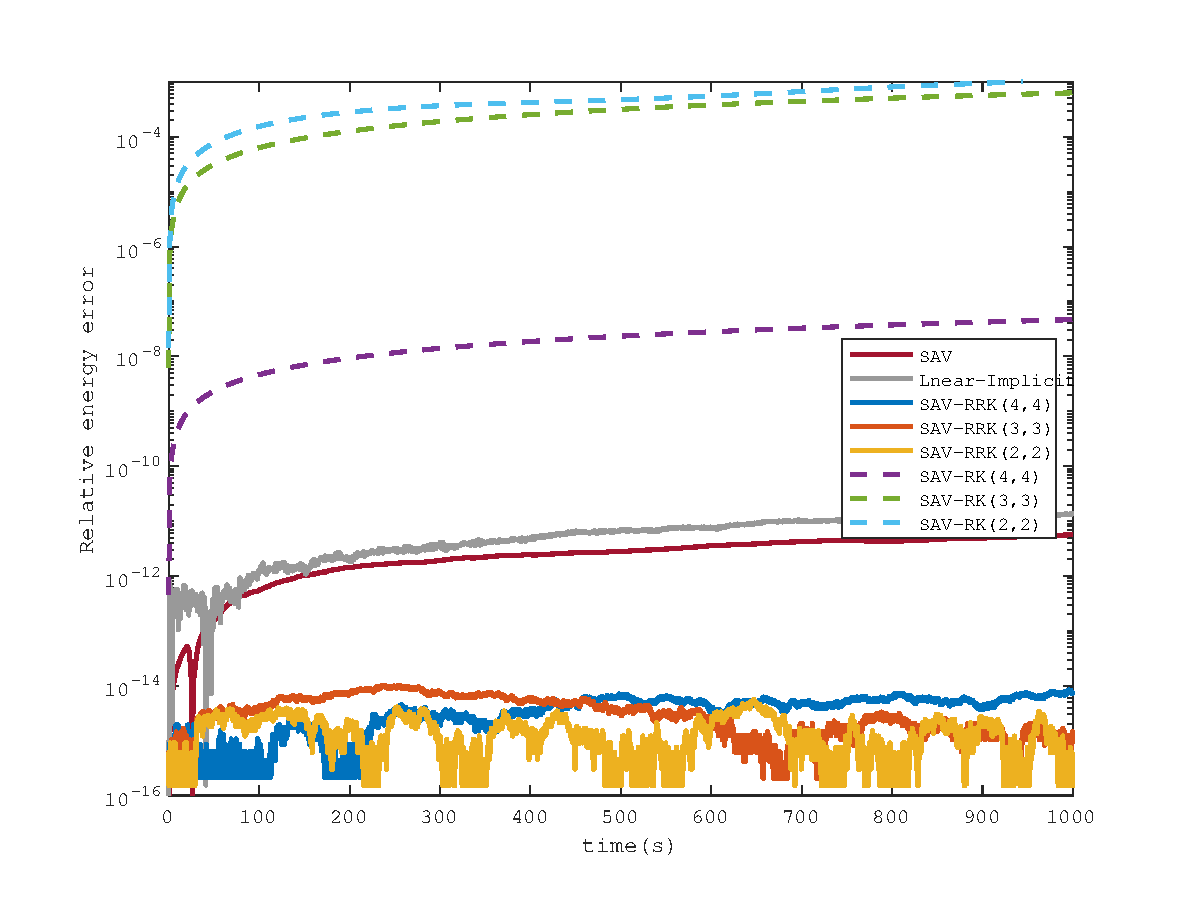
\includegraphics[width=0.35\textwidth]{./figure/exp1_energy9.eps}
		%\centerline{($b$) Spatial accuracy with $\tau = 10^{-3}.$}
		}\subfigure[$\alpha=2$]{ \centering
		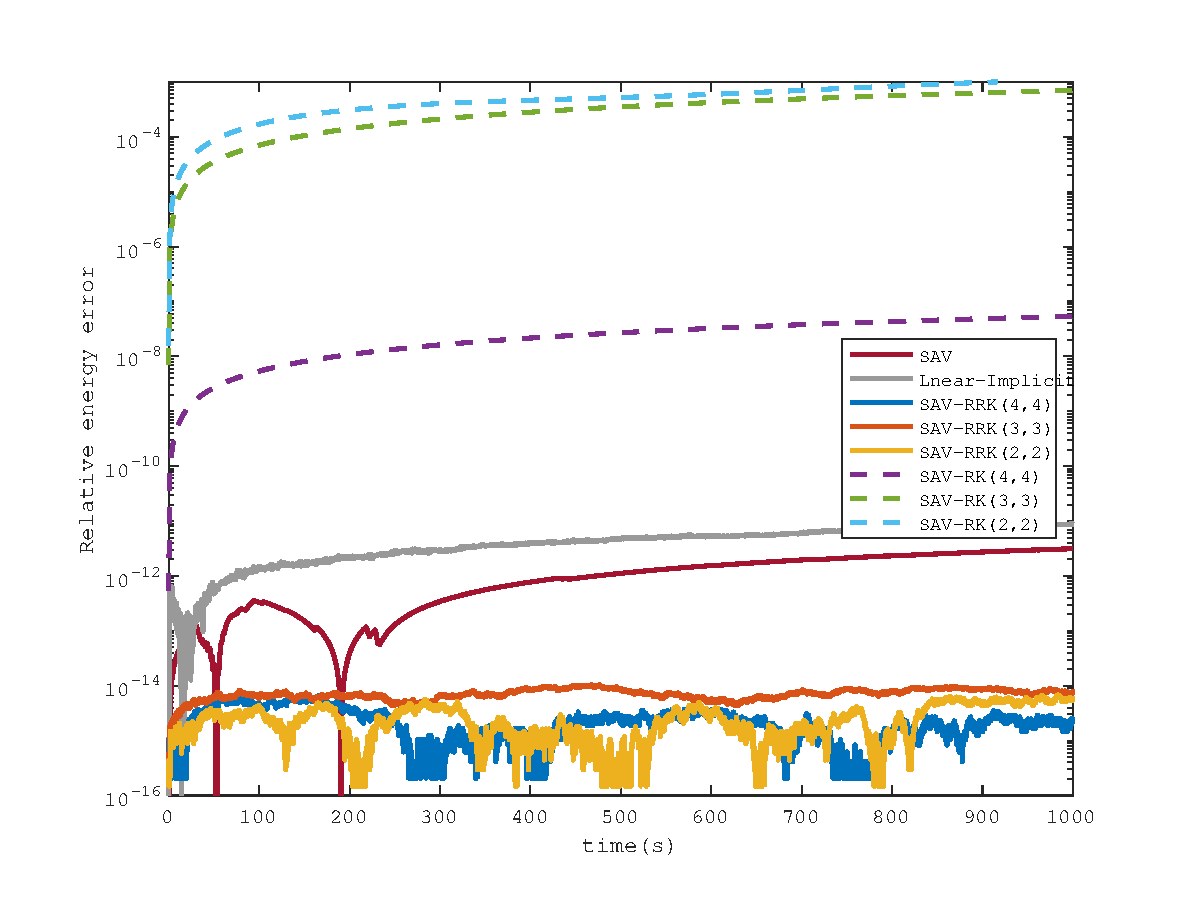
\includegraphics[width=0.35\textwidth]{./figure/exp1_energy2.eps}
		%\centerline{($a$) Temporal accuracy with $N=128.$}
		}\caption{ Relative errors of energy with $N=32, \tau=0.01$ for different $\alpha$ in Example \ref{ex:1}.}
		\label{fig:4}
		\end{center}
		\end{figure}
	\end{frame}
	
	\begin{frame}\frametitle{Numerical examples: 2D NFSWEs}
	\begin{example}\label{ex:2}
	  Now we consider the 2D NFSWEs \eqref{eq_1}-\eqref{eq_3} with initial values
	  \begin{align*}
		  u(x, y, 0)=\operatorname{sech}\left(x^2+y^2\right), u_t(x, y, 0)=\sin (x+y) \operatorname{sech}\left(-2\left(x^2+y^2\right)\right),
	  \end{align*}
	  where $(x, y, t) \in \Omega \times[0, T]$ and $\Omega=[-5,5] \times[-5,5]$.
	  \end{example}
	
	In order to reconfirm the applicability of the theoretical results in 2D case,
	  the same arguments as in Example \ref{ex:1} are considered in the calculation.
	  That is, $\alpha=1.5$ and $T=1$.  The obtained convergence order in temporal is presented in Table \ref{tab:6-2}. We can observe that the only difference
	  from the 1D case is that the SAV-RRK(IDT) methods do not achieve a higher-than-expected
	  order in the 2D case.
	\end{frame}
	
	\begin{frame}\frametitle{Numerical examples: 2D NFSWEs}
	\begin{table}[H]\tiny
	  \centering
	  \caption{Numerical errors and convergence order in time for Example \ref{ex:2} when $N=4, T = 1$.}
	  \begin{tabular}{lllllrlrlrlrlrl}
	  \toprule
	  \multicolumn{2}{l}{\multirow{2}[3]{*}{\textbf{RK(Stage,Order)}}} & \multicolumn{2}{l}{\multirow{2}[3]{*}{$\bm{\tau}$}} & \multicolumn{3}{c}{\textbf{SAV-RK}} &       & \multicolumn{3}{c}{\textbf{SAV-RRK}} &       & \multicolumn{3}{c}{\textbf{SAV-RRK(IDT)}} \\
	  \cmidrule{5-7}\cmidrule{9-11}\cmidrule{13-15}    \multicolumn{2}{l}{} & \multicolumn{2}{l}{} & \textbf{Error($\tau$)} &       & \textbf{order} &       & \textbf{Error($\tau$)} &       & \textbf{order} &       & \textbf{Error($\tau$)} &       & \textbf{order} \\
	  \hline
	  \multicolumn{2}{l}{\multirow{5}[0]{*}{\textbf{RK(2,2)}}} & \multicolumn{2}{l}{0.1} & 3.0217E-03 &       & -     &       & 3.0102E-03 &       & -     &       & 1.5692E-02 &       & - \\
	  \multicolumn{2}{l}{} & \multicolumn{2}{l}{0.05} & 7.4615E-04 &       & 2.0178  &       & 7.4702E-04 &       & 2.0106  &       & 9.6213E-03 &       & 0.7057  \\
	  \multicolumn{2}{l}{} & \multicolumn{2}{l}{0.025} & 1.8513E-04 &       & 2.0109  &       & 1.8587E-04 &       & 2.0069  &       & 5.2472E-03 &       & 0.8747  \\
	  \multicolumn{2}{l}{} & \multicolumn{2}{l}{0.0125} & 4.6090E-05 &       & 2.0060  &       & 4.6341E-05 &       & 2.0039  &       & 2.7312E-03 &       & 0.9420  \\
	  \multicolumn{2}{l}{} & \multicolumn{2}{l}{0.00625} & 1.1497E-05 &       & 2.0032  &       & 1.1569E-05 &       & 2.0021  &       & 1.3923E-03 &       & 0.9721  \\
	  \multicolumn{2}{l}{\multirow{5}[0]{*}{\textbf{RK(3,3)}}} & \multicolumn{2}{l}{0.1} & 1.2581E-04 &       & -     &       & 3.9379E-05 &       & -     &       & 3.2535E-03 &       & - \\
	  \multicolumn{2}{l}{} & \multicolumn{2}{l}{0.05} & 1.6180E-05 &       & 2.9589  &       & 5.5726E-06 &       & 2.8210  &       & 7.9304E-04 &       & 2.0365  \\
	  \multicolumn{2}{l}{} & \multicolumn{2}{l}{0.025} & 2.0532E-06 &       & 2.9783  &       & 7.4443E-07 &       & 2.9041  &       & 1.9546E-04 &       & 2.0205  \\
	  \multicolumn{2}{l}{} & \multicolumn{2}{l}{0.0125} & 2.5863E-07 &       & 2.9889  &       & 9.6210E-08 &       & 2.9519  &       & 4.8500E-05 &       & 2.0108  \\
	  \multicolumn{2}{l}{} & \multicolumn{2}{l}{0.00625} & 3.2454E-08 &       & 2.9944  &       & 1.2228E-08 &       & 2.9760  &       & 1.2078E-05 &       & 2.0056  \\
	  \multicolumn{2}{l}{\multirow{5}[1]{*}{\textbf{RK(4,4)}}} & \multicolumn{2}{l}{0.1} & 7.9185E-06 &       & -     &       & 8.0508E-06 &       & -     &       & 3.4013E-05 &       & - \\
	  \multicolumn{2}{l}{} & \multicolumn{2}{l}{0.05} & 4.9103E-07 &       & 4.0113  &       & 4.9644E-07 &       & 4.0194  &       & 3.3898E-06 &       & 3.3268  \\
	  \multicolumn{2}{l}{} & \multicolumn{2}{l}{0.025} & 3.0531E-08 &       & 4.0075  &       & 3.0805E-08 &       & 4.0104  &       & 3.6901E-07 &       & 3.1995  \\
	  \multicolumn{2}{l}{} & \multicolumn{2}{l}{0.0125} & 1.9026E-09 &       & 4.0042  &       & 1.9182E-09 &       & 4.0054  &       & 4.2681E-08 &       & 3.1120  \\
	  \multicolumn{2}{l}{} & \multicolumn{2}{l}{0.00625} & 1.1873E-10 &       & 4.0022  &       & 1.1966E-10 &       & 4.0027  &       & 5.1191E-09 &       & 3.0596  \\
	  \bottomrule
	  \end{tabular}%
	  \label{tab:6-2}%
	  \end{table}%
	\end{frame}
	
	%\begin{frame}
	%\begin{figure}[H]
	%  \begin{center}
	%  \subfigure[$\max _m\left|\gamma_m-1\right|$]{ \centering
	%  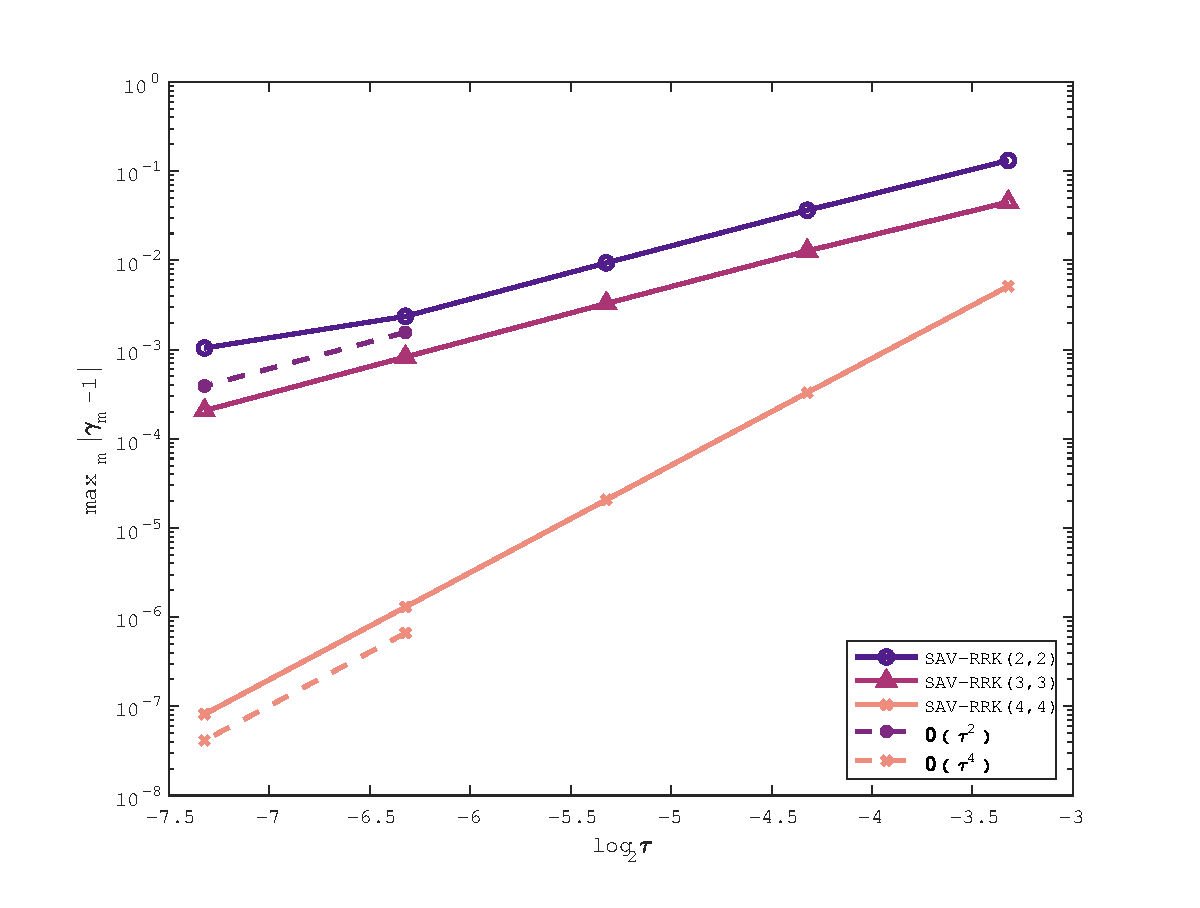
\includegraphics[width=0.5\textwidth]{./figure/exp2_r.eps}
	%  %\centerline{($b$) Spatial accuracy with $\tau = 10^{-3}.$}
	%  }\subfigure[$\max_m\left|S_m(1)\right|$]{ \centering
	%  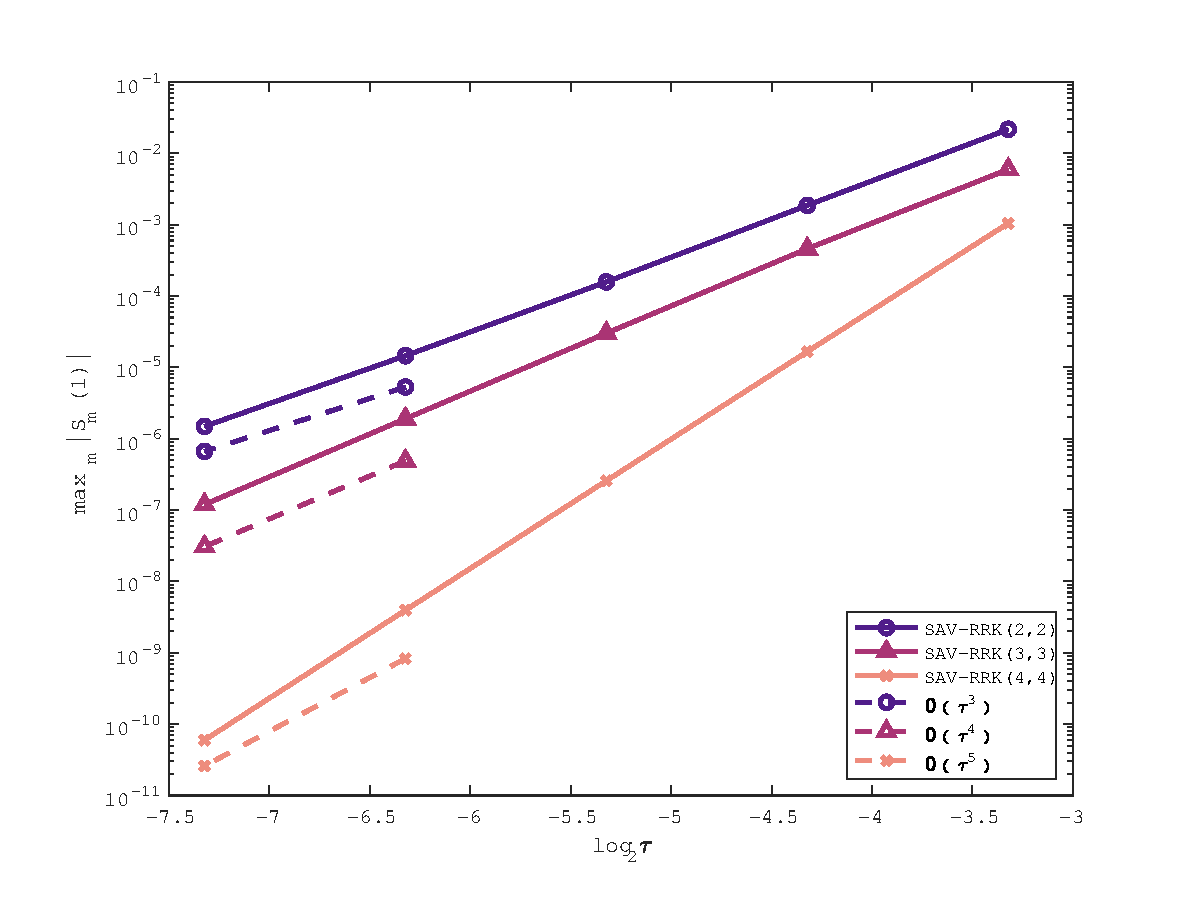
\includegraphics[width=0.5\textwidth]{./figure/exp2_s.eps}
	%  %\centerline{($a$) Temporal accuracy with $N=128.$}
	%  }\caption{$\max _m\left|\gamma_m-1\right|$ and $\max_m\left|S_m(1)\right|$ for some relaxation (RT) methods in Example \ref{ex:2}.}
	%  \label{fig:2-1}
	%  \end{center}
	%  \end{figure}
	%\end{frame}
	
	\begin{frame}\frametitle{Numerical examples: 2D NFSWEs}
	To demonstrate the effectiveness of the proposed methods in preserving
	energy, we perform long time simulations until $T=100$ and plot the
	relative energy errors using the SAV-RRK(4,4) methods with different
	$\alpha$ in Fig. \ref{fig:2-4}. The results reveal that the proposed methods can preserve energy exactly at the discrete level, and the
	conservation performance is significantly better than that of the SAV
	method \footnote{\tiny 	X.~Cheng, H.~Qin, J.~Zhang,
	\href{https://linkinghub.elsevier.com/retrieve/pii/S0377042721003848}{Convergence
	of an energy-conserving scheme for nonlinear space fractional
	{{Schr\"odinger}} equations with wave operator}, J. Comput. Appl. Math. 400
	(2022) 113762.}.
	\end{frame}
	
	\begin{frame}
	\vspace{-3mm}
	  \begin{figure}[H]
		\begin{center}
		\subfigure[$\alpha=1.3$]{ \centering
		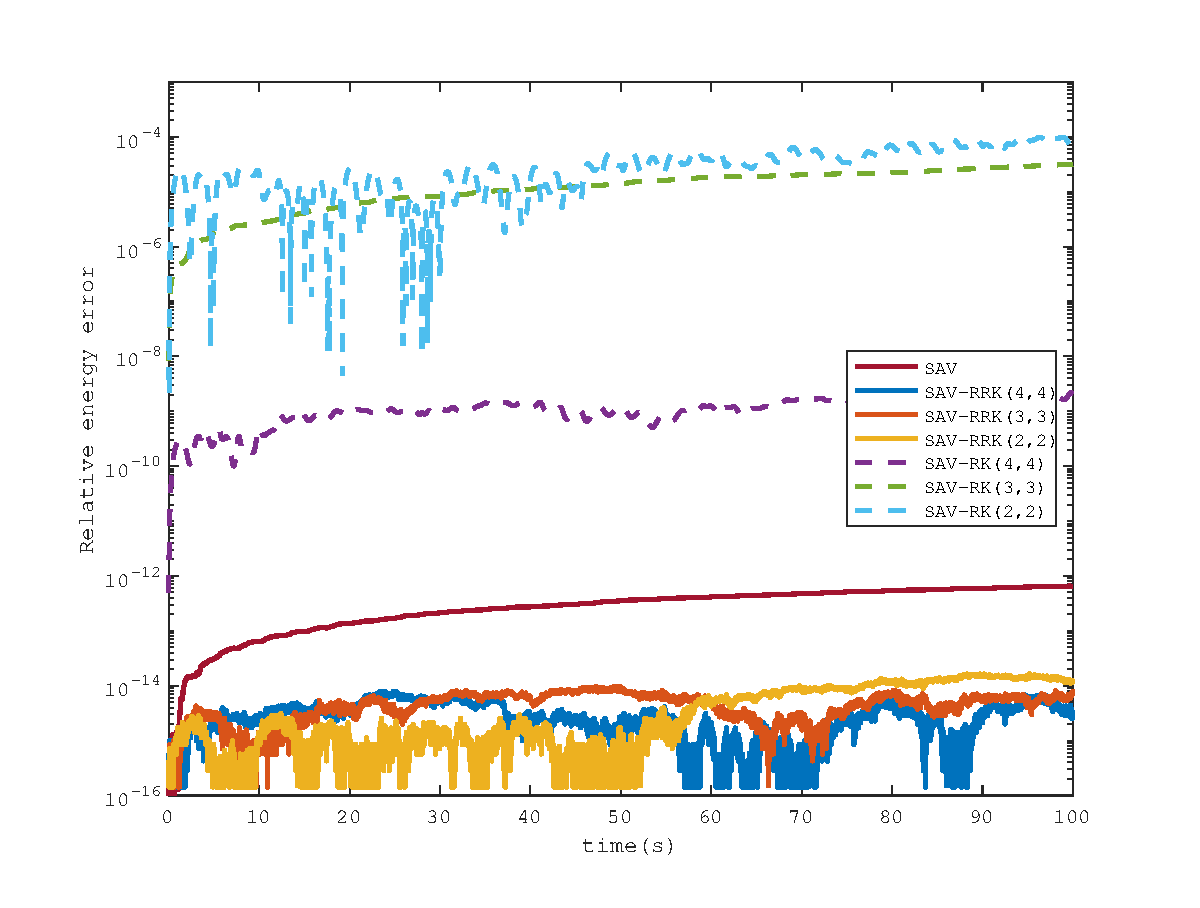
\includegraphics[width=0.35\textwidth]{./figure/exp2_energy3.eps}
		%\centerline{($b$) Spatial accuracy with $\tau = 10^{-3}.$}
		}\subfigure[$\alpha=1.6$]{ \centering
		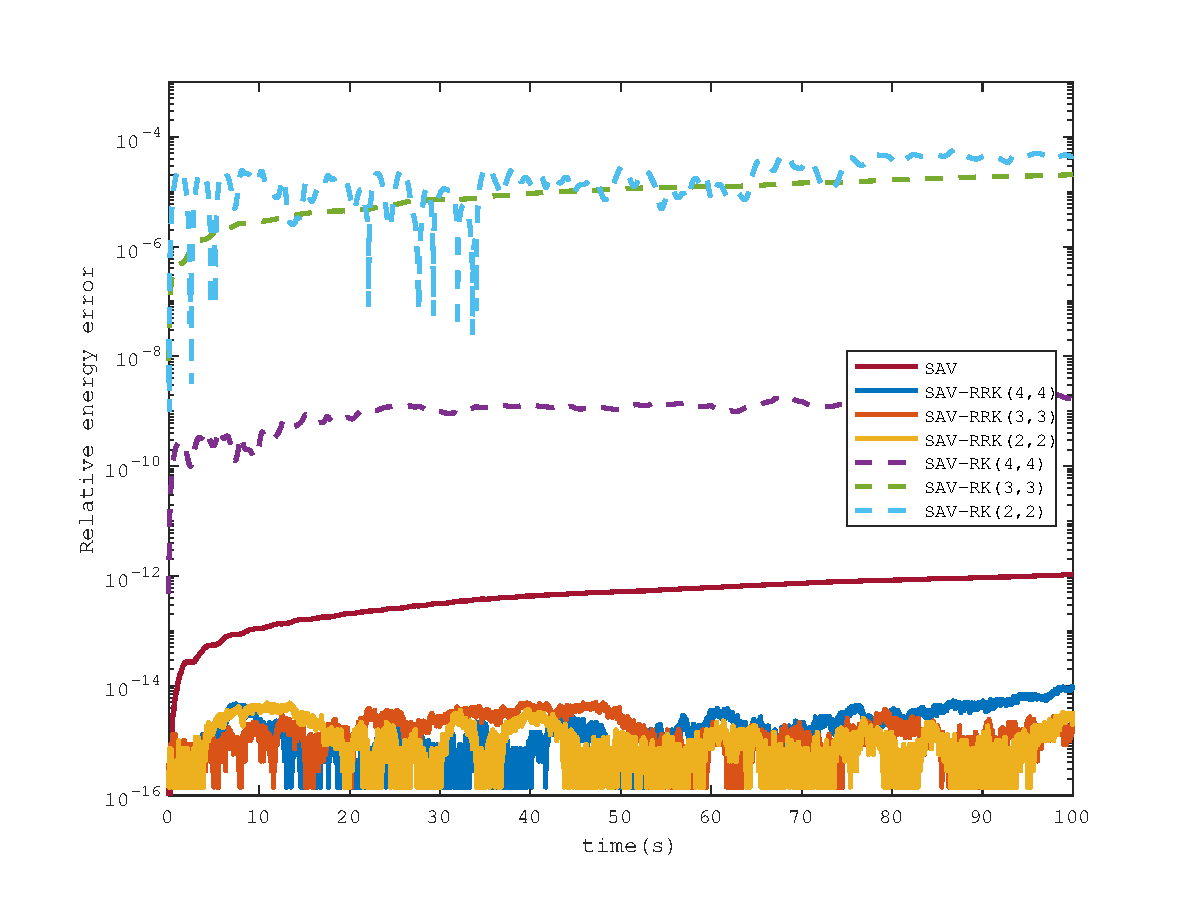
\includegraphics[width=0.35\textwidth]{./figure/exp2_energy6.eps}
		%\centerline{($a$) Temporal accuracy with $N=128.$}
		}\\\vspace{-3mm}
		\subfigure[$\alpha=1.9$]{ \centering
		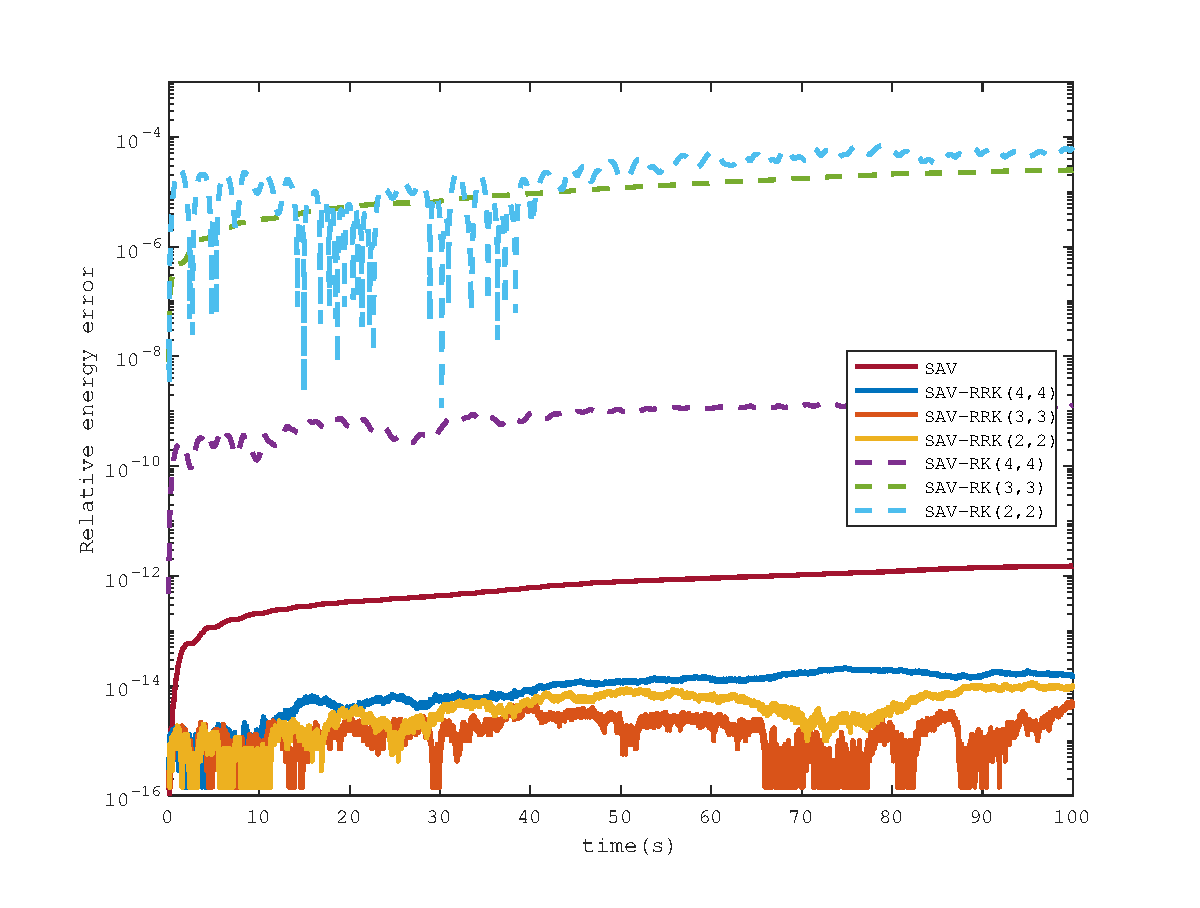
\includegraphics[width=0.35\textwidth]{./figure/exp2_energy9.eps}
		%\centerline{($b$) Spatial accuracy with $\tau = 10^{-3}.$}
		}\subfigure[$\alpha=2$]{ \centering
		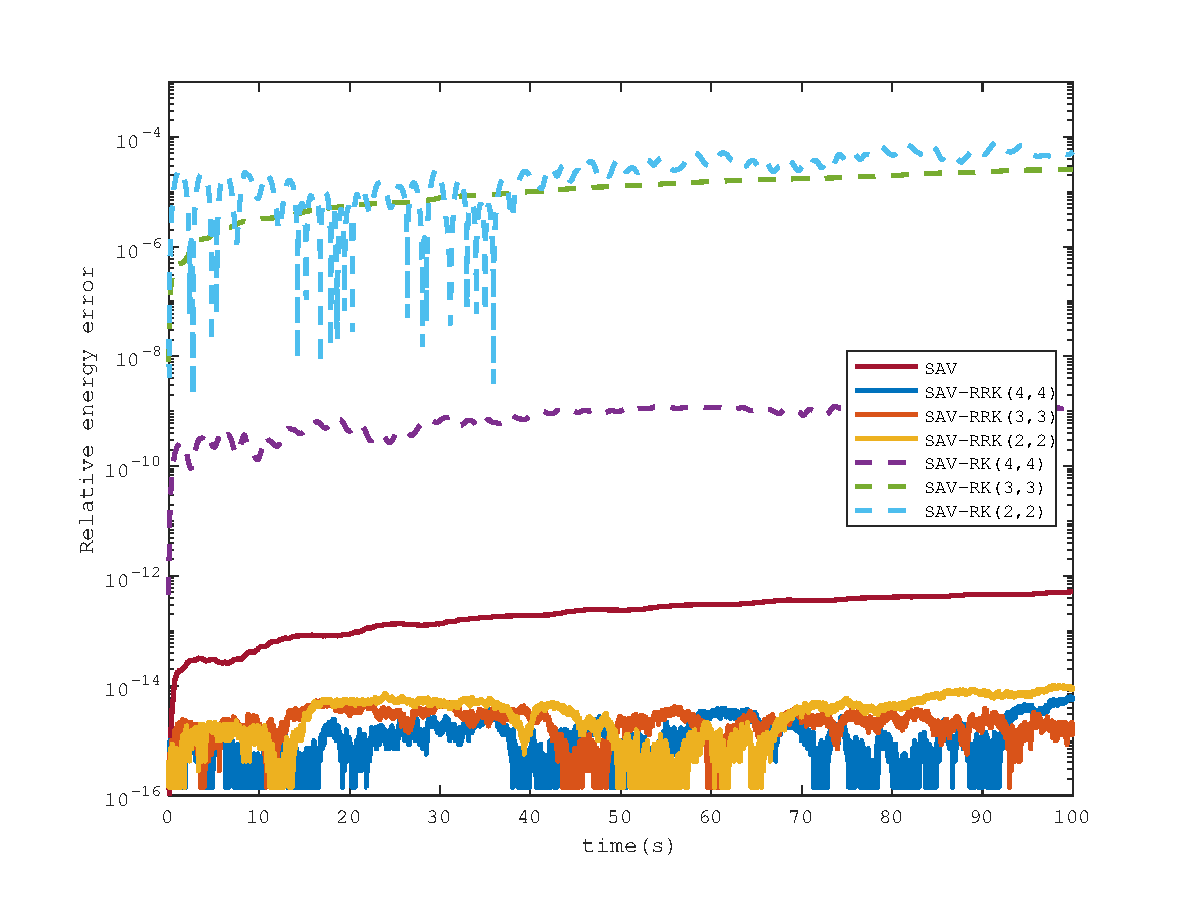
\includegraphics[width=0.35\textwidth]{./figure/exp2_energy2.eps}
		%\centerline{($a$) Temporal accuracy with $N=128.$}
		}\caption{ Relative errors of energy with $N=4, \tau=0.01$ for different $\alpha$ in Example \ref{ex:2}.}
		\label{fig:2-4}
		\end{center}
		\end{figure}
	\end{frame}
	
	\begin{frame}\frametitle{Numerical examples: 2D nonlinear fractional wave equation}
	\begin{example}\label{ex:3}
	  \footnote{\tiny N.~Wang, M.~Li, C.~Huang,
	  \href{https://link.springer.com/10.1007/s10915-021-01534-8}{Unconditional
	  {{Energy Dissipation}} and {{Error Estimates}} of the {{SAV Fourier Spectral
	  Method}} for {{Nonlinear fractional  wave equation}}}, J. Sci.
	  Comput. 88~(1) (2021) 19.} Next, we consider the 2D nonlinear fractional wave equation
	  \begin{equation}
	  \begin{cases}
	  & u_{t t}+(-\Delta)^{\frac{\alpha}{2}} u+F^{\prime}(u)=0,(x, y, t) \in \Omega \times(0, T],\\
	  & u(x, y, 0)=\frac{1}{2} \arctan \left(\exp \left(-\sqrt{x^2+y^2}\right)\right), u_t(x, y, 0)=0,
	  \end{cases}
	  \end{equation}
	  where $\Omega=(-10,10) \times(-10,10)$.
	  \end{example}
	
	Taking the potential energy $F(u)=u^2\left(\frac{1}{4} u^2-\frac{1}{2}\right)$. The convergence order
	  in time for $\alpha=1.5$ at $T=1$ is shown in Table \ref{tab:6-3}.
	  Also, the evolution of discrete energy for a long-time simulation ($T=100$) is depicted in Fig. \ref{fig:3-4}.
	  These data is calculated by applying the SAV-RRK(4,4) method. The results indicate that the proposed methods
	  is also valid for the nonlinear fractional wave equations.
	\end{frame}
	
	\begin{frame}\frametitle{Numerical examples: 2D nonlinear fractional wave equation}
	  \begin{table}[H]\tiny
		\centering
		\caption{Numerical errors and convergence order in time for Example \ref{ex:3} when $N=4, T = 1$.}
		\begin{tabular}{lllllrlrlrlrlrl}
		\toprule
		\multicolumn{2}{l}{\multirow{2}[3]{*}{\textbf{RK(Stage,Order)}}} & \multicolumn{2}{l}{\multirow{2}[3]{*}{$\bm{\tau}$}} & \multicolumn{3}{c}{\textbf{SAV-RK}} &       & \multicolumn{3}{c}{\textbf{SAV-RRK(RT)}} &       & \multicolumn{3}{c}{\textbf{SAV-RRK(IDT)}} \\
		\cmidrule{5-7}\cmidrule{9-11}\cmidrule{13-15}    \multicolumn{2}{l}{} & \multicolumn{2}{l}{} & \textbf{Error($\tau$)} &       & \textbf{order} &       & \textbf{Error($\tau$)} &       & \textbf{order} &       & \textbf{Error($\tau$)} &       & \textbf{order} \\
		\hline
		\multicolumn{2}{l}{\multirow{5}[0]{*}{\textbf{RK(2,2)}}} & \multicolumn{2}{l}{0.1} & 1.3395E-03 &       & -     &       & 3.3870E-03 &       & -     &       & 2.1470E-02 &       & - \\
		\multicolumn{2}{l}{} & \multicolumn{2}{l}{0.05} & 3.4360E-04 &       & 1.9628  &       & 8.1480E-04 &       & 2.0555  &       & 1.0960E-02 &       & 0.9701  \\
		\multicolumn{2}{l}{} & \multicolumn{2}{l}{0.025} & 8.6945E-05 &       & 1.9826  &       & 1.9951E-04 &       & 2.0300  &       & 5.5113E-03 &       & 0.9918  \\
		\multicolumn{2}{l}{} & \multicolumn{2}{l}{0.0125} & 2.1865E-05 &       & 1.9915  &       & 4.9347E-05 &       & 2.0154  &       & 2.7600E-03 &       & 0.9977  \\
		\multicolumn{2}{l}{} & \multicolumn{2}{l}{0.00625} & 5.4823E-06 &       & 1.9958  &       & 1.2270E-05 &       & 2.0078  &       & 1.3807E-03 &       & 0.9993  \\
		\multicolumn{2}{l}{\multirow{5}[0]{*}{\textbf{RK(3,3)}}} & \multicolumn{2}{l}{0.1} & 3.5168E-05 &       & -     &       & 4.3927E-05 &       & -     &       & 3.8213E-04 &       & - \\
		\multicolumn{2}{l}{} & \multicolumn{2}{l}{0.05} & 4.3533E-06 &       & 3.0141  &       & 5.4825E-06 &       & 3.0022  &       & 8.0473E-05 &       & 2.2475  \\
		\multicolumn{2}{l}{} & \multicolumn{2}{l}{0.025} & 5.3902E-07 &       & 3.0137  &       & 6.8378E-07 &       & 3.0032  &       & 1.8560E-05 &       & 2.1163  \\
		\multicolumn{2}{l}{} & \multicolumn{2}{l}{0.0125} & 6.7058E-08 &       & 3.0068  &       & 8.5344E-08 &       & 3.0022  &       & 4.4475E-06 &       & 2.0611  \\
		\multicolumn{2}{l}{} & \multicolumn{2}{l}{0.00625} & 8.3615E-09 &       & 3.0036  &       & 1.0659E-08 &       & 3.0012  &       & 1.0883E-06 &       & 2.0309  \\
		\multicolumn{2}{l}{\multirow{5}[1]{*}{\textbf{RK(4,4)}}} & \multicolumn{2}{l}{0.1} & 5.3561E-07 &       & -     &       & 3.2716E-06 &       & -     &       & 3.7745E-05 &       & - \\
		\multicolumn{2}{l}{} & \multicolumn{2}{l}{0.05} & 3.6438E-08 &       & 3.8777  &       & 2.0654E-07 &       & 3.9855  &       & 4.8050E-06 &       & 2.9737  \\
		\multicolumn{2}{l}{} & \multicolumn{2}{l}{0.025} & 2.3735E-09 &       & 3.9403  &       & 1.2898E-08 &       & 4.0012  &       & 6.0237E-07 &       & 2.9958  \\
		\multicolumn{2}{l}{} & \multicolumn{2}{l}{0.0125} & 1.5146E-10 &       & 3.9700  &       & 8.0476E-10 &       & 4.0024  &       & 7.5303E-08 &       & 2.9999  \\
		\multicolumn{2}{l}{} & \multicolumn{2}{l}{0.00625} & 9.5636E-12 &       & 3.9853  &       & 5.0241E-11 &       & 4.0016  &       & 9.4105E-09 &       & 3.0004  \\
		\bottomrule
		\end{tabular}%
		\label{tab:6-3}%
		\end{table}%
	\end{frame}
	
	\begin{frame}
	  \vspace{-3mm}
	  \begin{figure}[H]
		\begin{center}
		\subfigure[$\alpha=1.3$]{ \centering
		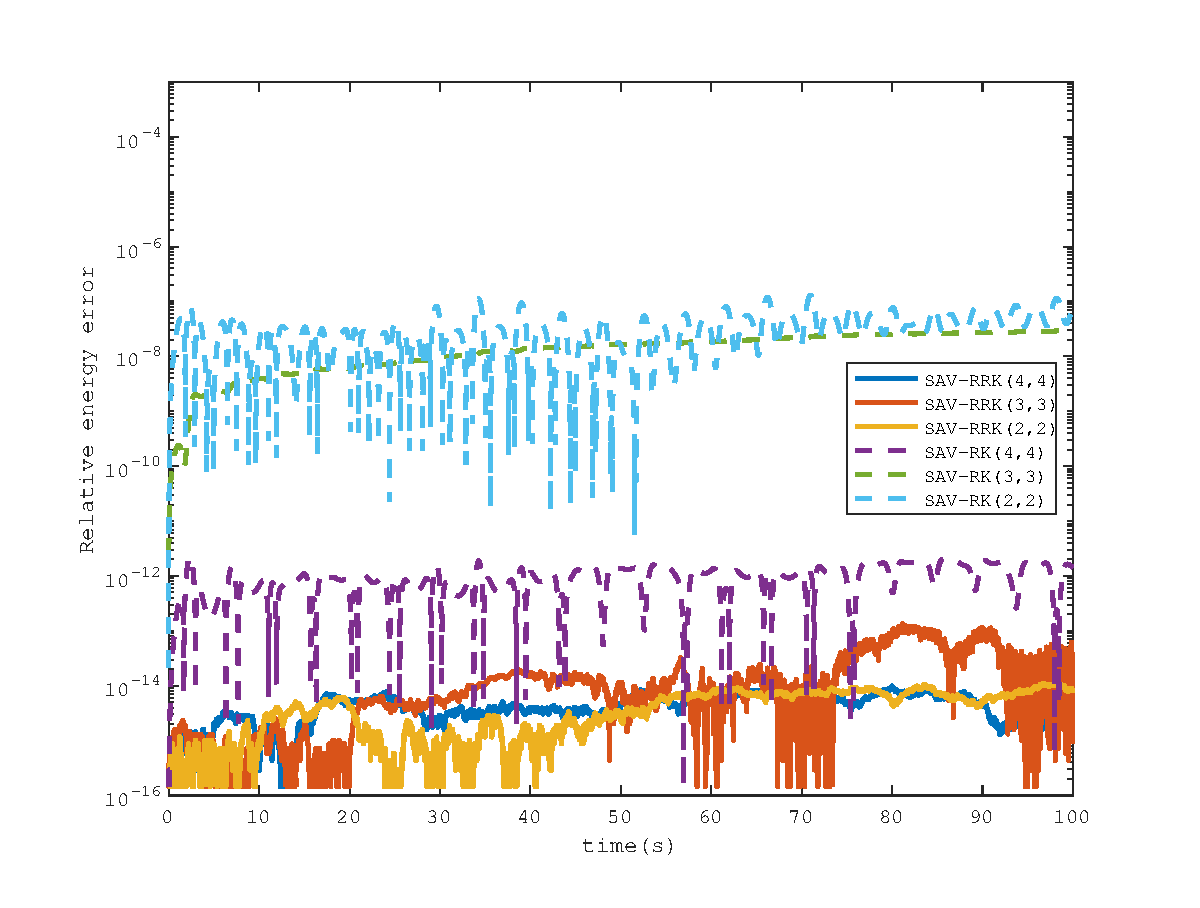
\includegraphics[width=0.35\textwidth]{./figure/exp3_energy3.eps}
		%\centerline{($b$) Spatial accuracy with $\tau = 10^{-3}.$}
		}\subfigure[$\alpha=1.6$]{ \centering
		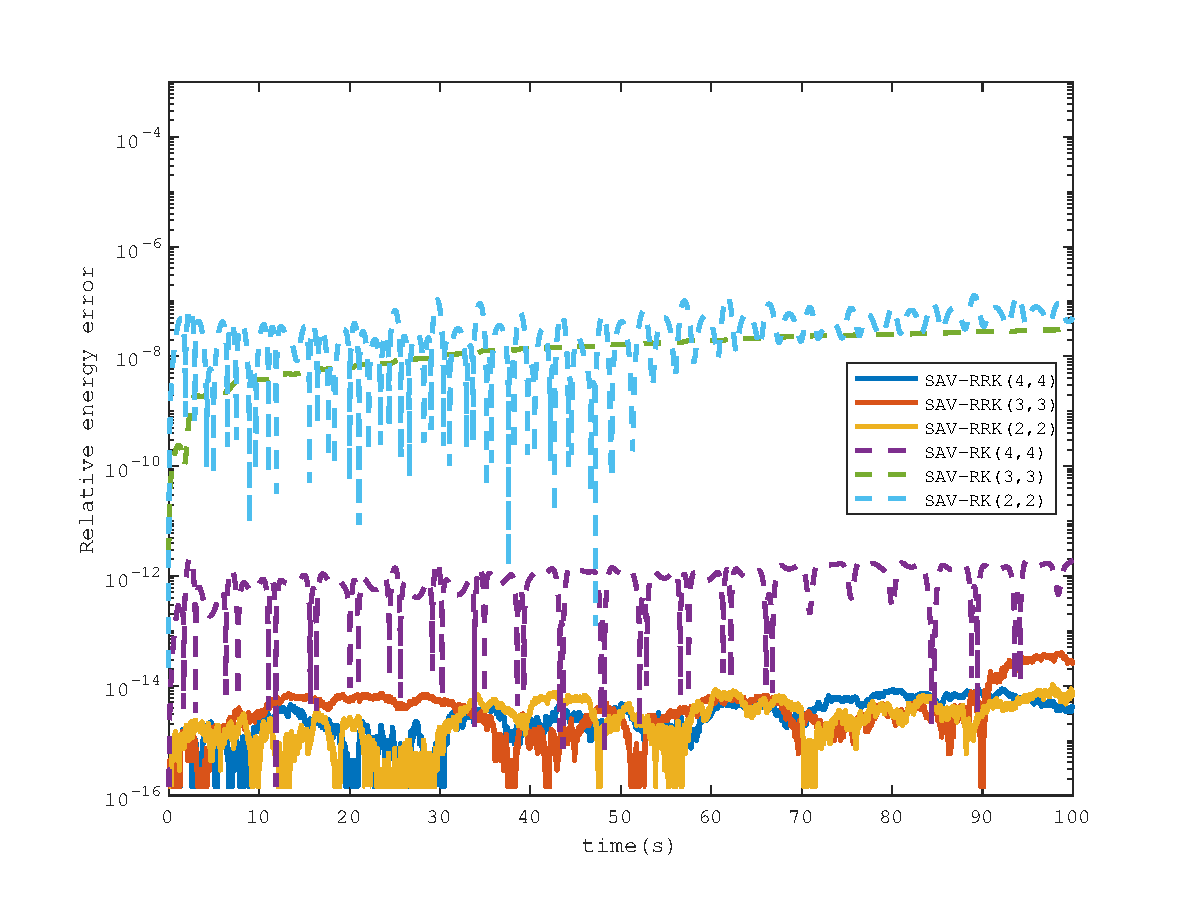
\includegraphics[width=0.35\textwidth]{./figure/exp3_energy6.eps}
		%\centerline{($a$) Temporal accuracy with $N=128.$}
		}\\\vspace{-3mm}
		\subfigure[$\alpha=1.9$]{ \centering
		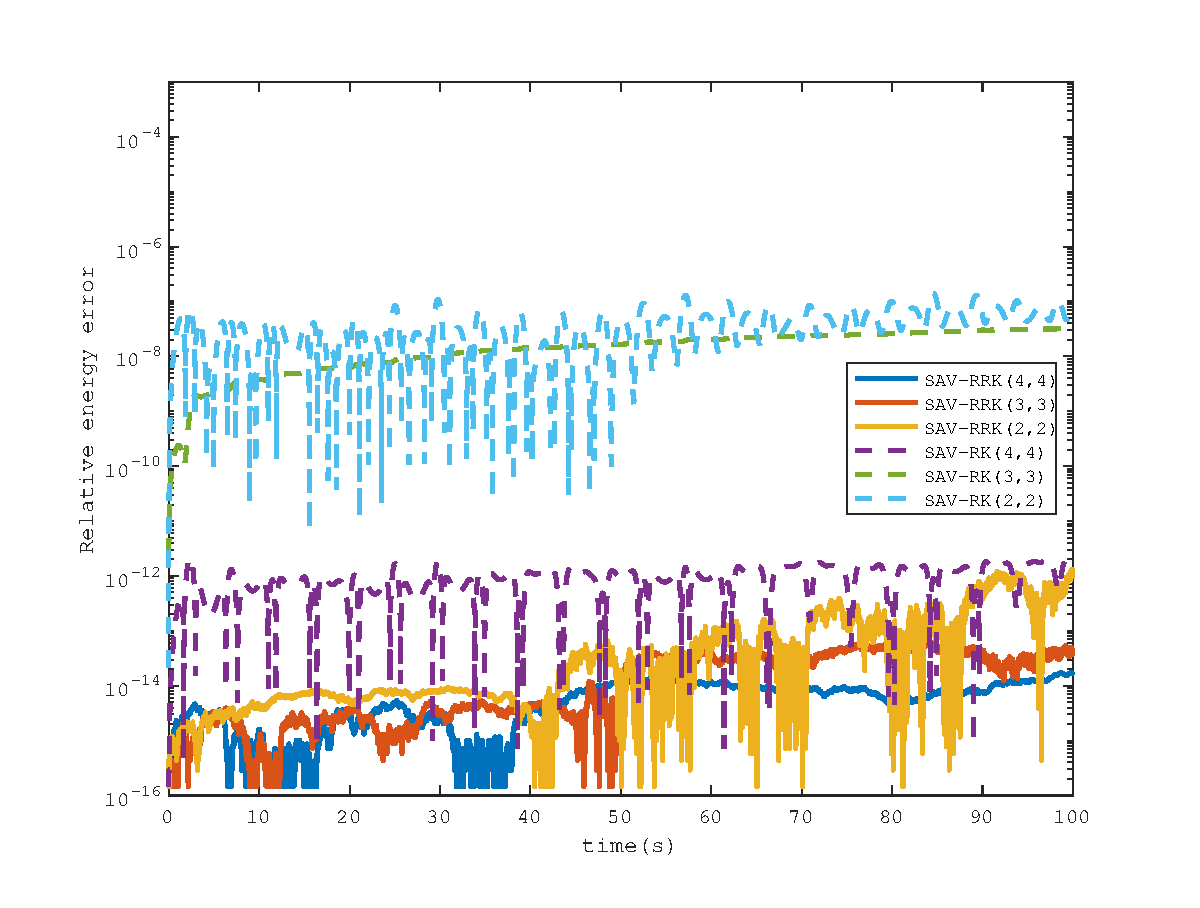
\includegraphics[width=0.35\textwidth]{./figure/exp3_energy9.eps}
		%\centerline{($b$) Spatial accuracy with $\tau = 10^{-3}.$}
		}\subfigure[$\alpha=2$]{ \centering
		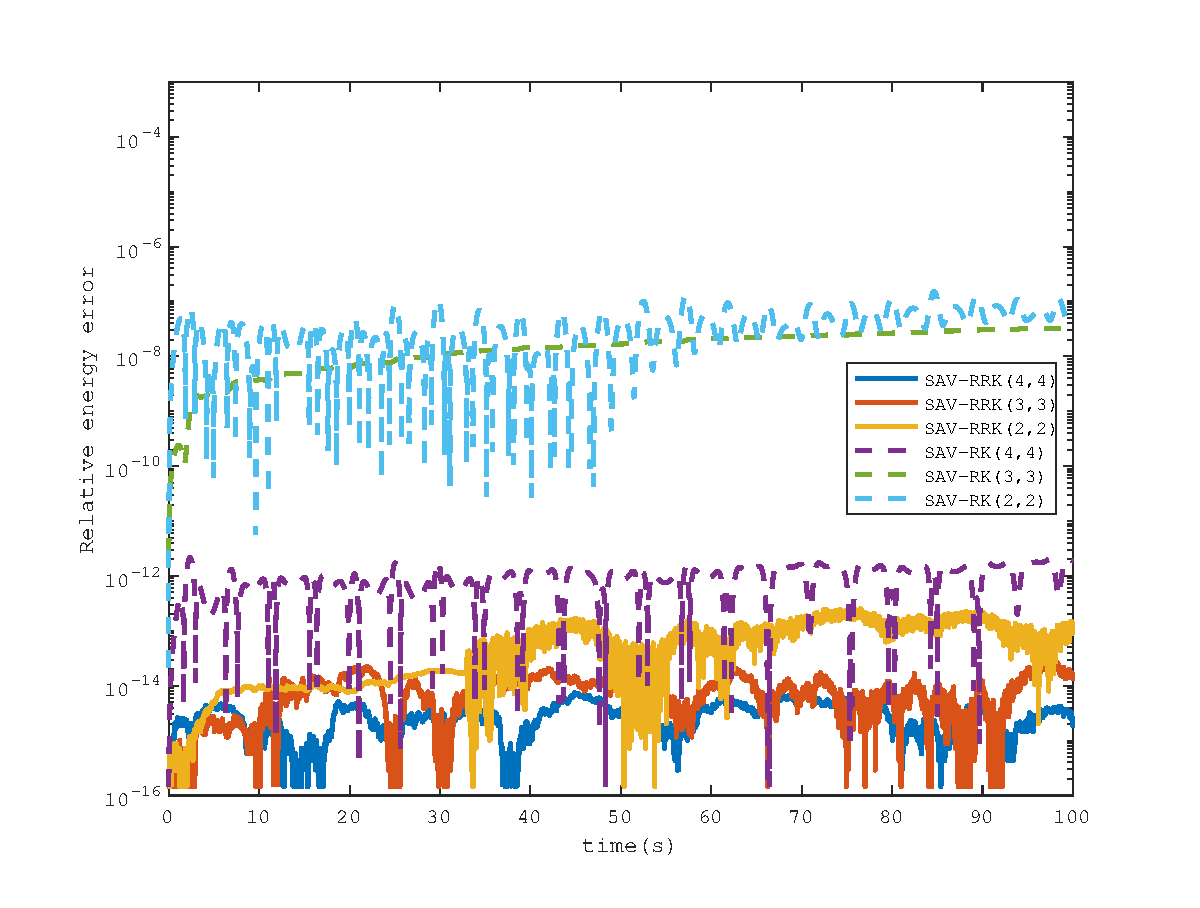
\includegraphics[width=0.35\textwidth]{./figure/exp3_energy2.eps}
		%\centerline{($a$) Temporal accuracy with $N=128.$}
		}\caption{ Relative errors of energy with $N=4, \tau=0.01$ for different $\alpha$ in Example \ref{ex:3}.}
		\label{fig:3-4}
		\end{center}
		\end{figure}
	\end{frame}
	
	\begin{frame}\frametitle{Numerical examples: 2D fractional KGS equation}
		\begin{example}\label{ex:4}
			\footnote{\tiny 	Y.~Fu, W.~Cai, Y.~Wang,
			\href{https://www.sciencedirect.com/science/article/pii/S0168927420301264}{Structure-preserving
			algorithms for the two-dimensional fractional {{Klein-Gordon-Schr\"odinger}}
			equation}, Appl. Numer. Math. 156 (2020) 77--93.}
			Finally, we consider the 2D fractional Klein-Gordon-Schr{\"o}dinger equation
			{\footnotesize\begin{equation}
			\begin{cases}
			\mathrm{i} \partial_t u-\frac{1}{2}(-\Delta)^{\frac{\alpha}{2}} u+u \phi=0,(x, y, t) \in \Omega \times(0, T],\\
			\partial_{t t} \phi+(-\Delta)^{\frac{\beta}{2}} \phi+\phi-|u|^2=0, (x, y, t) \in \Omega \times(0, T],
			\end{cases}
			\end{equation}}
			with the initial conditions
			{\footnotesize \begin{equation}
			\begin{aligned}
				&u(x, y, 0)=(1+\mathrm{i}) \exp \left(-|\boldsymbol{x}|^2\right),~~\phi(x, y, 0)=\operatorname{sech}\left(|\boldsymbol{x}|^2\right),\\
			& \partial_t \phi(x, y, 0)=\sin (x+y) \operatorname{sech}\left(-2|\boldsymbol{x}|^2\right),
			\end{aligned}
			\end{equation}}
			where $\Omega=[-10,10] \times[-10,10]$.
			\end{example}
		
		{\footnotesize Similar to the previous examples, some numerical errors and convergence order in time are listed in Table \ref{tab:6-4} for $\alpha=\beta=1.5$.}
		\end{frame}
	
	\begin{frame}\frametitle{Numerical examples: 2D fractional KGS equation}
	\begin{table}[H]\tiny
	  \centering
	  \caption{Numerical errors and convergence order in time for Example \ref{ex:4} when $N=4, T = 1$.}
	  \begin{tabular}{lllllrlrlrlrlrl}
	  \toprule
	  \multicolumn{2}{l}{\multirow{2}[3]{*}{\textbf{RK(Stage,Order)}}} & \multicolumn{2}{l}{\multirow{2}[3]{*}{$\bm{\tau}$}} & \multicolumn{3}{c}{\textbf{SAV-RK}} &       & \multicolumn{3}{c}{\textbf{SAV-RRK(RT)}} &       & \multicolumn{3}{c}{\textbf{SAV-RRK(IDT)}} \\
	  \cmidrule{5-7}\cmidrule{9-11}\cmidrule{13-15}    \multicolumn{2}{l}{} & \multicolumn{2}{l}{} & \textbf{Error($\tau$)} &       & \textbf{order} &       & \textbf{Error($\tau$)} &       & \textbf{order} &       & \textbf{Error($\tau$)} &       & \textbf{order} \\
	  \hline
	  \multicolumn{2}{l}{\multirow{5}[0]{*}{\textbf{RK(2,2)}}} & \multicolumn{2}{l}{0.1} & 1.1875E-03 &       & -     &       & 1.8837E-03 &       & -     &       & 9.5325E-03 &       & - \\
	  \multicolumn{2}{l}{} & \multicolumn{2}{l}{0.05} & 2.7648E-04 &       & 2.1026  &       & 5.0394E-04 &       & 1.9023  &       & 6.7134E-03 &       & 0.5058  \\
	  \multicolumn{2}{l}{} & \multicolumn{2}{l}{0.025} & 6.6514E-05 &       & 2.0555  &       & 1.3036E-04 &       & 1.9508  &       & 3.8805E-03 &       & 0.7908  \\
	  \multicolumn{2}{l}{} & \multicolumn{2}{l}{0.0125} & 1.6300E-05 &       & 2.0288  &       & 3.3151E-05 &       & 1.9754  &       & 2.0757E-03 &       & 0.9026  \\
	  \multicolumn{2}{l}{} & \multicolumn{2}{l}{0.00625} & 4.0339E-06 &       & 2.0146  &       & 8.3587E-06 &       & 1.9877  &       & 1.0723E-03 &       & 0.9529  \\
	  \multicolumn{2}{l}{\multirow{5}[0]{*}{\textbf{RK(3,3)}}} & \multicolumn{2}{l}{0.1} & 8.7748E-05 &       & -     &       & 1.9567E-04 &       & -     &       & 3.1789E-03 &       & - \\
	  \multicolumn{2}{l}{} & \multicolumn{2}{l}{0.05} & 1.1471E-05 &       & 2.9354  &       & 2.4630E-05 &       & 2.9900  &       & 8.2646E-04 &       & 1.9435  \\
	  \multicolumn{2}{l}{} & \multicolumn{2}{l}{0.025} & 1.4684E-06 &       & 2.9657  &       & 3.0916E-06 &       & 2.9940  &       & 2.1079E-04 &       & 1.9712  \\
	  \multicolumn{2}{l}{} & \multicolumn{2}{l}{0.0125} & 1.8580E-07 &       & 2.9824  &       & 3.8731E-07 &       & 2.9968  &       & 5.3231E-05 &       & 1.9854  \\
	  \multicolumn{2}{l}{} & \multicolumn{2}{l}{0.00625} & 2.3370E-08 &       & 2.9911  &       & 4.8471E-08 &       & 2.9983  &       & 1.3375E-05 &       & 1.9927  \\
	  \multicolumn{2}{l}{\multirow{5}[1]{*}{\textbf{RK(4,4)}}} & \multicolumn{2}{l}{0.1} & 3.0741E-06 &       & -     &       & 4.0627E-06 &       & -     &       & 1.0278E-04 &       & - \\
	  \multicolumn{2}{l}{} & \multicolumn{2}{l}{0.05} & 1.9959E-07 &       & 3.9450  &       & 2.6020E-07 &       & 3.9647  &       & 1.3195E-05 &       & 2.9615  \\
	  \multicolumn{2}{l}{} & \multicolumn{2}{l}{0.025} & 1.2698E-08 &       & 3.9744  &       & 1.6461E-08 &       & 3.9825  &       & 1.6711E-06 &       & 2.9811  \\
	  \multicolumn{2}{l}{} & \multicolumn{2}{l}{0.0125} & 8.0044E-10 &       & 3.9876  &       & 1.0350E-09 &       & 3.9913  &       & 2.1024E-07 &       & 2.9906  \\
	  \multicolumn{2}{l}{} & \multicolumn{2}{l}{0.00625} & 5.0238E-11 &       & 3.9939  &       & 6.4882E-11 &       & 3.9957  &       & 2.6365E-08 &       & 2.9953  \\
	  \bottomrule
	  \end{tabular}%
	  \label{tab:6-4}%
	  \end{table}%
	\end{frame}
	
	\begin{frame}\frametitle{Numerical examples: 2D fractional KGS equation}
	Furthermore, the relative energy with different $\alpha$ and $\beta$ in a long-time simulation up to $T=100$ is described in Fig. \ref{fig:3-5}.
	  % The phenomenon shown by the image shows that the proposed schemes can accurately preserve energy in the discrete level for the fractional Klein-Gordon-Schr{\"o}dinger equation.
	  The phenomenon depicted demonstrates that the proposed methods accurately preserve energy at the discrete level for the fractional Klein-Gordon-Schr{\"o}dinger equation.
	\end{frame}
	
	\begin{frame}
	\vspace{-3mm}
	  \begin{figure}[H]
		\begin{center}
		\subfigure[$\alpha,\beta=1.3$]{ \centering
		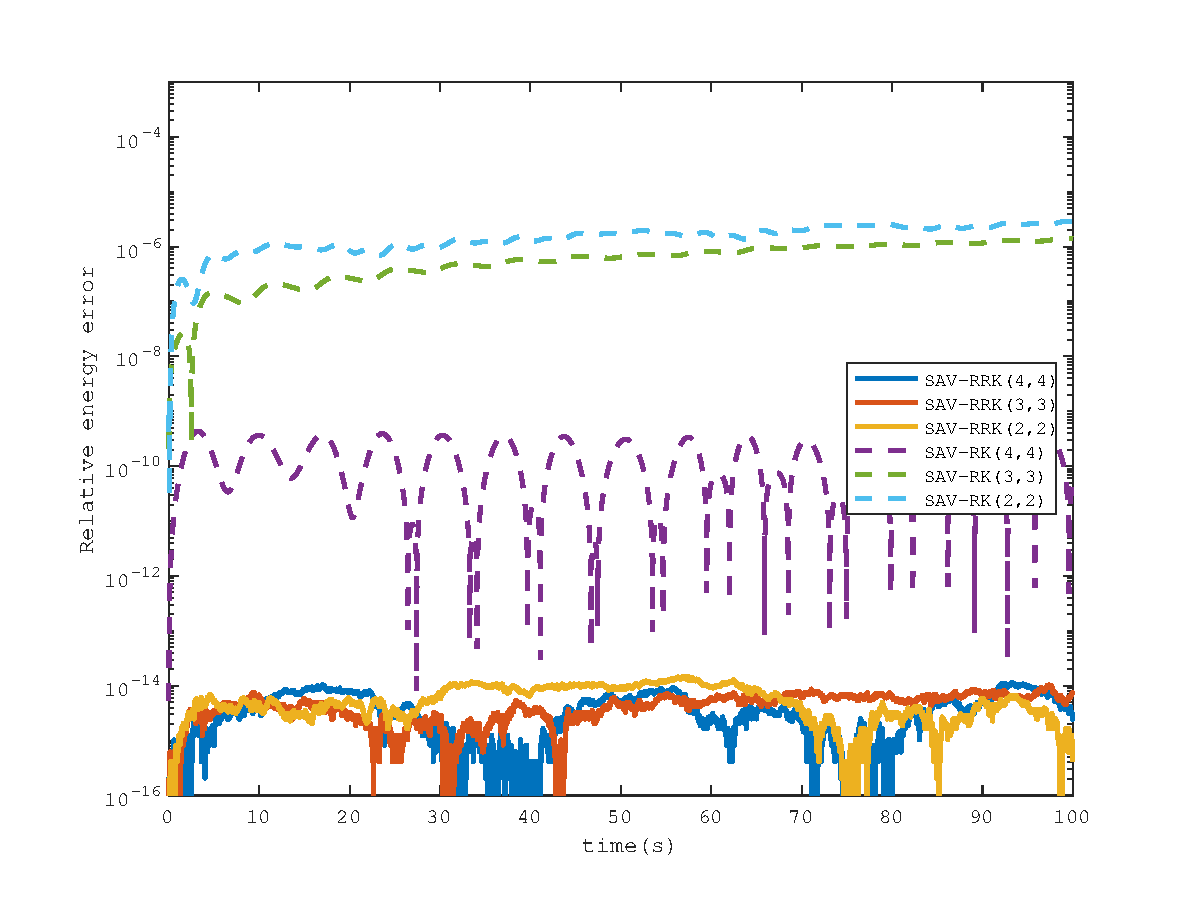
\includegraphics[width=0.35\textwidth]{./figure/exp4_energy3.eps}
		%\centerline{($b$) Spatial accuracy with $\tau = 10^{-3}.$}
		}\subfigure[$\alpha,\beta=1.6$]{ \centering
		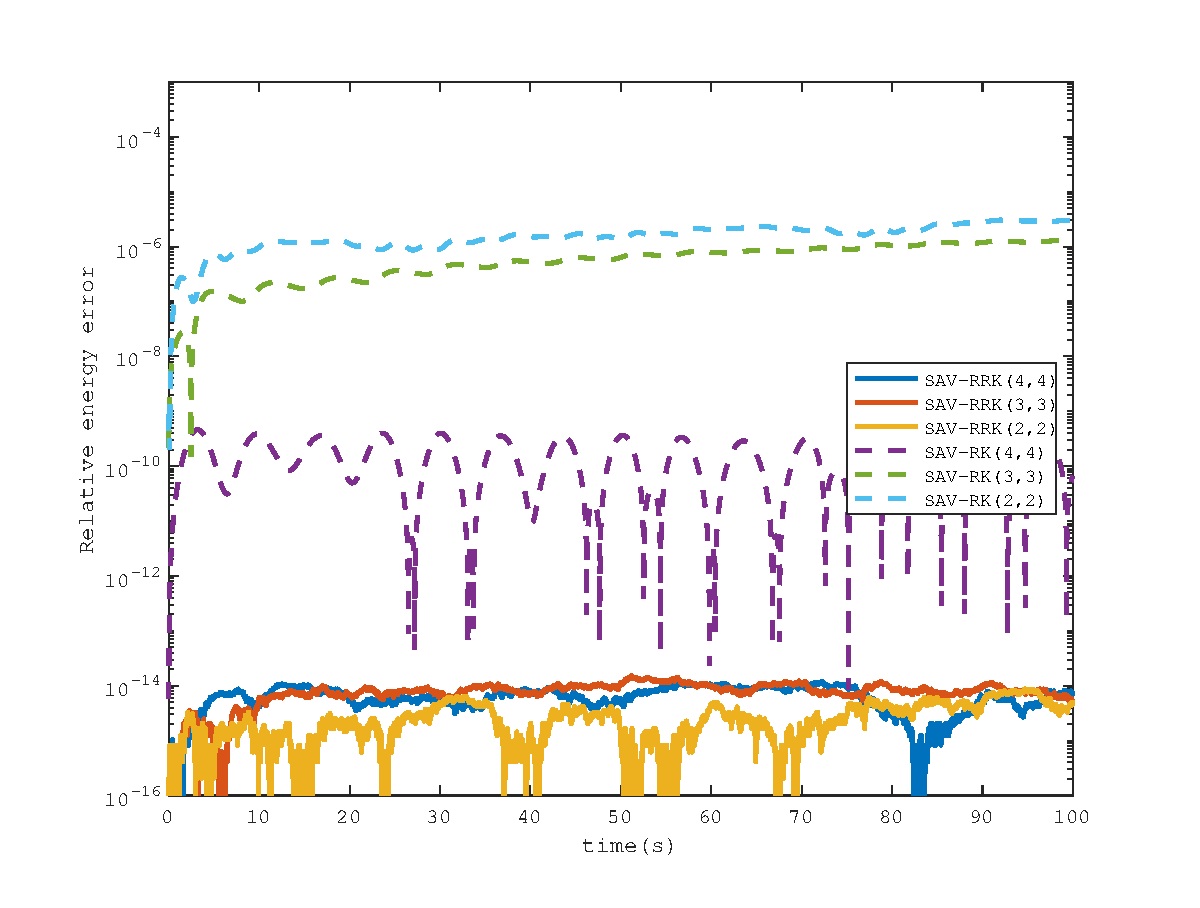
\includegraphics[width=0.35\textwidth]{./figure/exp4_energy6.eps}
		%\centerline{($a$) Temporal accuracy with $N=128.$}
		}\\\vspace{-3mm}
		\subfigure[$\alpha,\beta=1.9$]{ \centering
		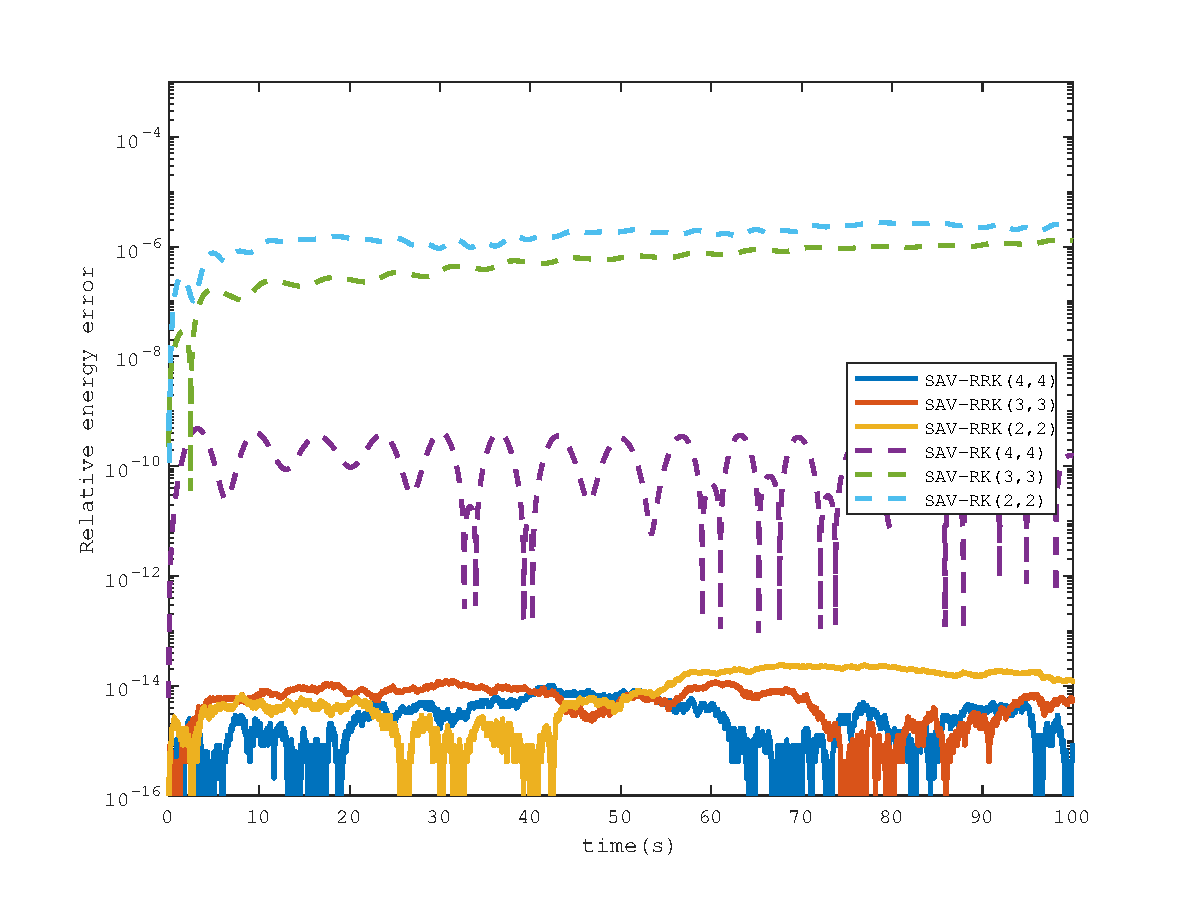
\includegraphics[width=0.35\textwidth]{./figure/exp4_energy9.eps}
		%\centerline{($b$) Spatial accuracy with $\tau = 10^{-3}.$}
		}\subfigure[$\alpha,\beta=2$]{ \centering
		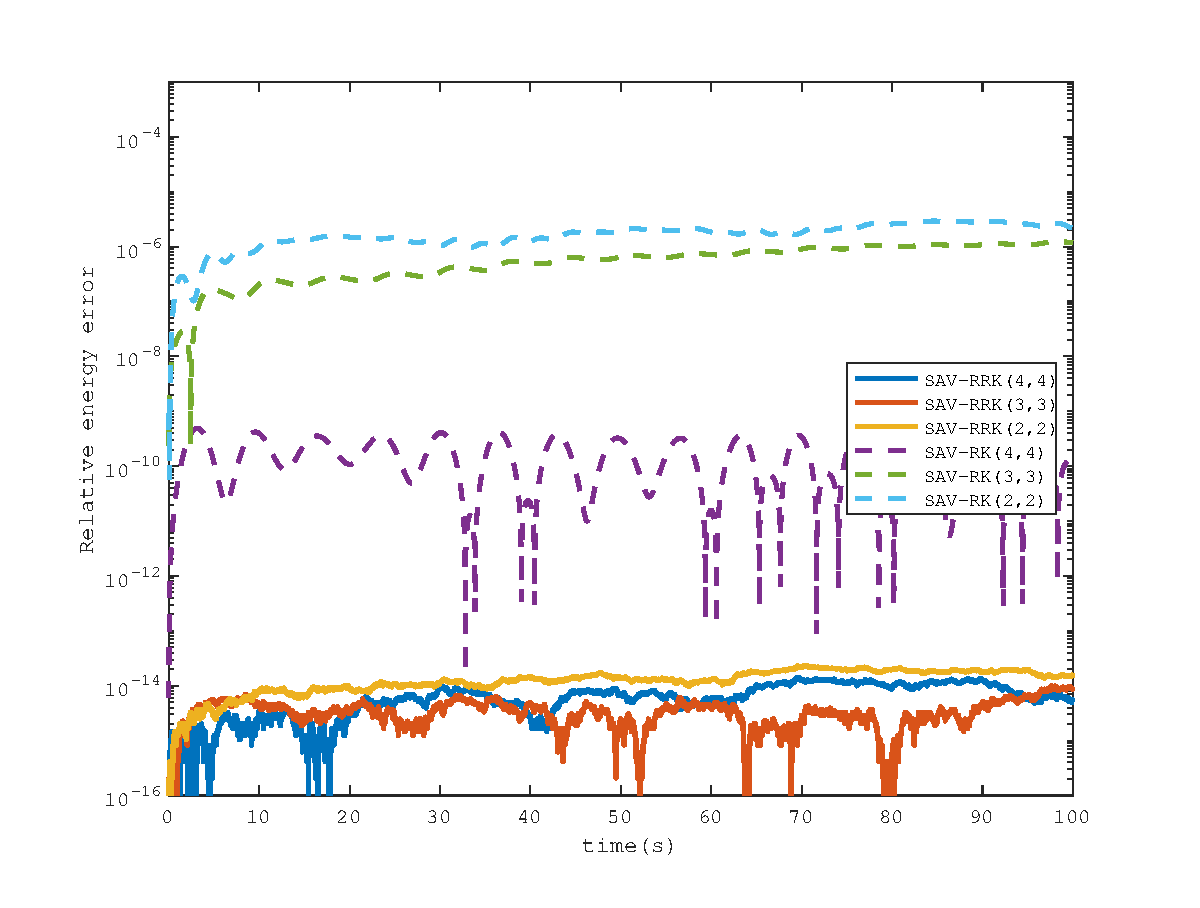
\includegraphics[width=0.35\textwidth]{./figure/exp4_energy2.eps}
		%\centerline{($a$) Temporal accuracy with $N=128.$}
		}\caption{ Relative errors of energy with $N=4, \tau=0.01$ for different $\alpha$ in Example \ref{ex:4}.}
		\label{fig:3-5}
		\end{center}
		\end{figure}
	\end{frame}

\section{总结展望}
\begin{frame}{总结展望}
	\begin{block}{本文总结}
			\begin{itemize}
				\item \textcolor[rgb]{0.227,0.373,0.306}{SAV-RRK:} 通过SAV方法将NFSWEs的非二次能量转化为新变量的二次形式,结合显式RK方法和松弛技术,提出了一种任意高阶的显式保结构数值格式。
				\item \textcolor[rgb]{0.227,0.373,0.306}{FPAVF-P:} 成功推导了具有周期边界条件的二维NFSWEs的哈密顿形式,引入了分区平均向量场(PAVF)方法,并采用PAVF-P方法构建了能够同时守恒原始能量和质量的数值格式。
				\item \textcolor[rgb]{0.227,0.373,0.306}{谱方法:} 本文使用了傅里叶拟谱方法,作为空间离散方法,充分利用了其非局部性质和傅里叶基函数的特性,通过快速傅里叶变换(FFT)提高了计算效率。
			\end{itemize}
			% 综合而言,本文在NFSWEs数值求解方面取得了新的研究成果,提出的方法在长时间仿真具有良好的适用性,为未来相关研究提供了有益的参考。
		\end{block}
		
\end{frame}

\begin{frame}{课题的创新性}
	\begin{block}{创新性}
		% {\footnotesize 本课题的创新点不仅体现在方法的创新,还体现在对物理问题的深入研究和建模上,对相关领域的研究和发展具有一定的推动作用.}
		\begin{itemize}
			\item {\footnotesize 本课题拟利用分数阶Laplacian函数的变分原理,推导二维NFSWEs的\textbf{\textcolor[rgb]{0.227,0.373,0.306}{哈密顿结构}},为后续研究提供新的思路和方法.}
			\item {\footnotesize 本课题将为 NFSWEs 构造如下两种保结构算法}
		\end{itemize}
	\begin{table}[htbp]
		\centering
		% \caption{本课题的目标是为二维NFSWEs构建高效的显式保结构格式以及能够同时保持原始能量和质量的格式}
		  \begin{tabular}{cccccc}
		  \toprule
		  \textcolor[rgb]{0.227,0.373,0.306}{} & \textcolor[rgb]{0.227,0.373,0.306}{\textbf{维度}} & \textcolor[rgb]{0.227,0.373,0.306}{\textbf{空间精度}} & \textcolor[rgb]{0.227,0.373,0.306}{\textbf{时间精度}} & \textcolor[rgb]{0.227,0.373,0.306}{\textbf{能量守恒}} & \textcolor[rgb]{0.227,0.373,0.306}{\textbf{质量守恒}} \\
		  \midrule
		  \textcolor[rgb]{0.227,0.373,0.306}{\textbf{格式-1}} & \textcolor{purple}{2 维}   & \textcolor{purple}{谱精度}   & \textcolor{purple}{任意高阶}  & 修正能量  & 无 \\
		  \midrule
		  \textcolor[rgb]{0.227,0.373,0.306}{\textbf{格式-2}} & \textcolor{purple}{2 维}   & \textcolor{purple}{谱精度}   & 2 阶   & \textcolor{purple}{原始能量}  & \textcolor{purple}{原始质量} \\
		  \bottomrule
		  \end{tabular}%
		\label{tab:3}%
	  \end{table}%
	\end{block}
	\end{frame}
\begin{frame}{总结展望}
	\begin{block}{研究展望}
		% {\footnotesize }
		在本文的基础上及研究过程中, 发现存在以下改进空间:
		\begin{enumerate}
			\item \textcolor[rgb]{0.227,0.373,0.306}{推广到高维问题:}目前研究主要集中在二维问题的差分格式上, 未来可将这些方法推广至更高维度, 如三维或更高维度的非线性分数阶薛定谔方程.
			\item \textcolor[rgb]{0.227,0.373,0.306}{深入分析稳定性和收敛性:}对数值方法的收敛性及稳定性尚未进行充分的分析. 对提出的数值方法, 需要进行更深入的稳定性和收敛性分析, 以验证其可靠性和有效性.
			\item \textcolor[rgb]{0.227,0.373,0.306}{探索新的数值方法和模型:}未来的研究可以探索并应用新的数值方法和模型, 如神经网络方法或深度学习方法, 以解决非线性分数阶薛定谔方程的数值求解问题.
		\end{enumerate}
	\end{block}
\end{frame}
	
\section{参考文献}

\begin{frame}[allowframebreaks]
	% \tiny
	\scriptsize
	% \footnotesize
% \bibliographystyle{elsarticle-num} 
% \bibliography{/Users/dasha/Zotero/BetterBibTeX/mylibrary.bib}

\begin{thebibliography}{10}
	\expandafter\ifx\csname url\endcsname\relax
	  \def\url#1{\texttt{#1}}\fi
	\expandafter\ifx\csname urlprefix\endcsname\relax\def\urlprefix{URL }\fi
	\expandafter\ifx\csname href\endcsname\relax
	  \def\href#1#2{#2} \def\path#1{#1}\fi
	
	\bibitem{ranLinearlyImplicitConservative2016}
	M.~Ran, C.~Zhang,
	  \href{http://www.tandfonline.com/doi/full/10.1080/00207160.2015.1016924}{A
	  linearly implicit conservative scheme for the fractional nonlinear
	  {{Schr\"odinger}} equation with wave operator}, Int. J. Comput. Math. 93~(7)
	  (2016) 1103--1118.
 
	\bibitem{liFastEnergyConserving2018}
	M.~Li, Y.-L. Zhao,
	  \href{https://linkinghub.elsevier.com/retrieve/pii/S0096300318304983}{A fast
	  energy conserving finite element method for the nonlinear fractional
	  {{Schr\"odinger}} equation with wave operator}, Appl. Math. Comput. 338
	  (2018) 758--773.
 
	\bibitem{panFourthorderDifferenceScheme2022}
	K.~Pan, J.~Zeng, D.~He, S.~Zhang,
	  \href{https://doi.org/10.1080/00036811.2020.1829600}{A fourth-order
	  difference scheme for the fractional nonlinear {{Schr\"odinger}} equation
	  with wave operator}, Appl. Anal. 101~(8) (2022) 2886--2902.
	 
	\bibitem{chengConvergenceEnergyconservingScheme2022}
	X.~Cheng, H.~Qin, J.~Zhang,
	  \href{https://linkinghub.elsevier.com/retrieve/pii/S0377042721003848}{Convergence
	  of an energy-conserving scheme for nonlinear space fractional
	  {{Schr\"odinger}} equations with wave operator}, J. Comput. Appl. Math. 400
	  (2022) 113762.
 
	\bibitem{huEfficientEnergyPreserving2022}
	D.~Hu, W.~Cai, X.-M. Gu, Y.~Wang,
	  \href{https://linkinghub.elsevier.com/retrieve/pii/S0168927421002981}{Efficient
	  energy preserving {{Galerkin}}\textendash{{Legendre}} spectral methods for
	  fractional nonlinear {{Schr\"odinger}} equation with wave operator}, Appl.
	  Numer. Math. 172 (2022) 608--628.
 
	\bibitem{zhangHighorderStructurepreservingDifference2023}
	X.~Zhang, M.~Ran, Y.~Liu, L.~Zhang,
	  \href{https://www.sciencedirect.com/science/article/pii/S0378475423001325}{A
	  high-order structure-preserving difference scheme for generalized fractional
	  {{Schr\"odinger}} equation with wave operator}, Math. Comput. Simulation 210
	  (2023) 532--546.
 
	\bibitem{ketchesonRelaxationRungeKutta2019}
	D.~I. Ketcheson,
	  \href{https://epubs.siam.org/doi/abs/10.1137/19M1263662}{Relaxation
	  {{Runge--Kutta Methods}}: {{Conservation}} and {{Stability}} for
	  {{Inner-Product Norms}}}, SIAM J. Numer. Anal. 57~(6) (2019) 2850--2870.
 
	% \bibitem{ranochaRelaxationRungeKutta2020}
	% H.~Ranocha, M.~Sayyari, L.~Dalcin, M.~Parsani, D.~I. Ketcheson,
	%   \href{https://epubs.siam.org/doi/10.1137/19M1263480}{Relaxation
	%   {{Runge--Kutta Methods}}: {{Fully Discrete Explicit Entropy-Stable Schemes}}
	%   for the {{Compressible Euler}} and {{Navier--Stokes Equations}}}, SIAM J.
	%   Sci. Comput. 42~(2) (2020) A612--A638.
	 
	\bibitem{yangLinearUnconditionallyEnergy2017}
	X.~Yang, L.~Ju,
	  \href{https://www.sciencedirect.com/science/article/pii/S0045782516317856}{Linear
	  and unconditionally energy stable schemes for the binary fluid\textendash
	  surfactant phase field model}, Comput. Methods Appl. Mech. Eng. 318 (2017)
	  1005--1029.
 
	\bibitem{yangEfficientLinearSchemes2017}
	X.~Yang, L.~Ju,
	  \href{https://www.sciencedirect.com/science/article/pii/S0045782516306016}{Efficient
	  linear schemes with unconditional energy stability for the phase field
	  elastic bending energy model}, Comput. Methods Appl. Mech. Eng. 315 (2017)
	  691--712.
 
	\bibitem{caiPartitionedAveragedVector2018}
	W.~Cai, H.~Li, Y.~Wang,
	  \href{https://linkinghub.elsevier.com/retrieve/pii/S0021999118303012}{Partitioned
	  averaged vector field methods}, J. Comput. Phys. 370 (2018) 25--42.
 
	\bibitem{wangStructurepreservingNumericalMethods2018}
	P.~Wang, C.~Huang,
	  \href{https://linkinghub.elsevier.com/retrieve/pii/S0168927418300709}{Structure-preserving
	  numerical methods for the fractional {{Schr\"odinger}} equation}, Appl.
	  Numer. Math. 129 (2018) 137--158.
 
	\bibitem{fuStructurepreservingAlgorithmsTwodimensional2020}
	Y.~Fu, W.~Cai, Y.~Wang,
	  \href{https://www.sciencedirect.com/science/article/pii/S0168927420301264}{Structure-preserving
	  algorithms for the two-dimensional fractional {{Klein-Gordon-Schr\"odinger}}
	  equation}, Appl. Numer. Math. 156 (2020) 77--93.
 
	\end{thebibliography}
	
\end{frame}

\begin{frame}
\begin{center}
{\Huge\calligra \textbf{\textcolor[rgb]{0.227,0.373,0.306}{恳请各位专家批评指正!}}}
\end{center}
\end{frame}

\end{document}